% This file is responsible to collect all content and assemble the document.

% Edit these lines...
\def\thesisType{Master Thesis}
\def\name{HAKKEL Tamás}
\def\Program{Computer Science Engineering MSc}
\def\title{Iteratively Reweighted Algorithms for Dynamic MRI}
\def\supervisors{Supervisor: Claudio M. VERDUN \\ Faculty mentor: Dr. OLÁH András}

% ---------------------------------------------

% Render title page
\titlePage

% Set page numbering to roman numbers for all pages before the first chapter. Change it to "\pagenumbering{Roman}" if you want upper case roman numbers
\pagenumbering{roman}

% Mandatory parts
% If you don't want these mandatory parts to be included in the table of contents, simply delete or comment out the lines starting with "\addcontentsline".
\addcontentsline{toc}{chapter}{Diploma Thesis Proposal}

% If you print your thesis two sided, the you need this blank page after the Title page
\blankPage

% The "Diploma Thesis Proposal" form takes the first two page numbers, so the "Thesis Authenticity Statement" gets the page number 3.
\setcounter{page}{3}

\addcontentsline{toc}{chapter}{Thesis Authenticity Statement}
% You have nothing to do here

\chapter*{Thesis Authenticity Statement}
I, undersigned \name, student of the Faculty of Information Technology and Bionics at the Pázmány Péter Catholic University, hereby certify that this thesis was written without any unauthorized help, solely by me and I used only the referenced sources. Every part, which is quoted exactly or in a paraphrased manner, is indicated clearly with a reference. I have not submitted this thesis anywhere else.

% Signature line
\begin{flushright}
	\vspace*{.5cm}\par\noindent\makebox[2.5in]{\hrulefill}
	\par\noindent\makebox[2.5in][c]{\name}
\end{flushright}

\clearpage
\addcontentsline{toc}{chapter}{Abstract}
\chapter*{Abstract}

Although MR imagig was invented less then 50 years ago, it has revolutionized medical imaging and diagnostic process as we know it. Its versatility makes it fit a wide range of use cases, and compared to other imaging technologies, MRI demonstrates important advantages in many cases, such as lack of ionizing radiation, adjustable contrast range, and excellent differentiation between soft tissues. However, it has also a disadvantage: the imaging speed is undesirably slow. While it is only inconvenience in some cases, dynamic images of chest, for example, gets blurred by the different motions of the body, like breathing and cardiac motion. There are new technologies that improves the imaging process itself, but strong image reconstruction algorithms can vastly improve the quality.

Among the many software techniques invented to improve image quality, compressed sensing is inevitably is one of the most impactful theoretical construction, introduced by Donoho, Candès, Romberg, and Tao in 2004~\cite{candes_robust_2006, donoho_compressed_2006, candes_nearoptimal_2006}. In contrast to the Nyquist-Shannon theorem that asserts that continuous band-limited signals can be perfectly reconstructed from samples taken at a rate of twice the highest frequency present in the signal of interest, compressed sensing allows lossless reconstruction from much lower number of samples given that certain natural conditions are satisfied.

In this thesis work, we consider the classic results as well as the recent advances within of the compressed sensing framework and their application to real life MR imaging. In particular, we closely examine two recent publications presenting state-of-the-art solutions combining conventional techniques with novel ideas.

Afterwards, we present our implementation of these algorithms along with the implementation of a recently invented algorithm from the family of iteratively reweighted least squares (IRLS) methods that previously have not been applied to MRI setting yet. For the language of implementation we have chosen Julia, a new open-source language released in 2012, as this language fits well the image reconstruction problem being inherently fast with a speed often comparable to C, and providing convenient environment for fast prototyping.

Finally, we compare these algorithm with respect to reconstruction power from massively undersampled data and noise tolerance. Our results demonstrates the fitness of the Julia language to prototyping and also shows strong benchmark suggesting that a robust extension of the new IRLS method can bring enormous improvement to reconstruction quality or imaging speed.

\clearpage
% Uncomment the following line if you want to include an "Acknowledgements" page after the abstract.
%\addcontentsline{toc}{chapter}{Acknowledgements}
%\chapter*{Acknowledgements}
% Optional part to give thanks to people contributing to your work (other than your supervisor and mentor) https://seleninevcilikhayati.com/accounting-dissertation-help/

\paragraph{}
\lipsum[2] % 1 paragraph of dummy text - replace it with your thanksgiving lines
\clearpage

% Render table of contents
\tableofcontents
\clearpage

% From here page numbers are arabic numbers starting again from 1
\pagenumbering{arabic}

% Include files holding the content of your thesis -- feel free to change as you like it
\chapter{Introduction}\label{chapter:introduction}

While the fast evolution of technology profoundly changed today's medicine, unarguably the medical imaging is of the fields which profited the most of the computation power recently became available. And as X-rays revolutionized medical treatments in the beginning of the 20th century, after its discovery by Wilhelm Conrad Röntgen,  the appearance of computer-aided imaging techniques such as computer tomography (CT), diagnostic ultrasonography, positron emission tomography (PET), and magnetic resonance imaging (MRI) opened a new horizon drastically increasing the resolution, allowing 3D imaging, providing reliable dynamic recordings, and enhancing images by automated post-processing \cite{mri_picturetoproton}. In the recent decades radiology evolved to be an interdisciplinary field involving, for instance, molecular biology, nuclear physics, applied mathematics, and computer science besides the classical medical fields such as anatomy, angiology, and cardiology.

\section{Magnetic Resonance Imaging}

In particular, MRI has revolutionized medical imaging and diagnostic process as we know it. Its versatility makes it fit a wide range of use cases. Compared to other imaging technologies, MRI demonstrates important advantages in many cases.
\begin{itemize}
    \item In contrast to X-ray, MRI doesn't use any ionizing radiation, and hence it is totally harmless to the patient. Also, MRI has enhanced resolution for soft tissues compared to any other modality, in particular neural tissue,  while X-rays are rather used for diagnosing bone degeneration, dislocation, fracture or some tissue infection. Furthermore, MRI allows 3D scans. Nevertheless, MRI scanners are slow and expensive compare to X-ray scan machines and therefore hardware and software improvements are necessary for its wider use.
    \item As CT scanning is based on X-rays, it shares the downside with X-rays, doctors need to evaluate the possible benefits of the scan and decide if it outweighs the potential complications of exposure to ionizing radiations. MRI, however, elicit this problem, although at the price of a elongated imaging process. Comparing the medical problems where these technologies are used, one can conclude that CT scan is very helpful in diagnosing severe injuries of the chest, head, spine or abdomen, particularly fractures, and it is commonly used to localize tumors. MRI often performs better at diagnosing problems in the joints, soft tissues, ligaments and tendons. When available, doctors use it frequently to scan the spine, brain, muscles, neck, breasts, and abdomen.
    \item MRI still does not have the portability, low cost, and real-time imaging speed without any harmful radiation of ultrasound technology, but ultrasound is mostly limited to 2D imaging (although 3D imaging is possible), have trouble penetrating bone, and even in absence of bone the depth of penetration is limited depending on the frequency of imaging. This is not the case for MRI technology.
    \item PET scans are particularly useful for functional imaging. For instance, it is used for identification of lapses in cognitive function, examination of cardiac failures, cancer screening and diagnosis, and finding an infection.  Nevertheless, PET image acquisition is even longer than MRI (especially, if we consider also the time while patients wait for the tracer to reach the targeted organ), it uses a radioactive substance as tracer, and it cannot scan tissues not absorbing the tracer making the localization of the source of the signal infeasible without any additional information. In order to solve the latter described limitation, one particularly promising combination is the join use of PET and MRI. This illustrates that MRI is a fundamental technology not only by itself but also when combined with other imaging modalities.
\end{itemize}
To sum up, MRI is a strong competitor to other imaging technologies, but it also have weaknesses, of which the costs and scanning time are the most remarkable. There are many methods to speed up measurements as it will be discussed later, but the construction cost and the hardware constraints limit the applicability of these efforts. The problem of slowness is even more apparent in case of dynamic images as motion of organs (e.g. heart or lung) can drastically degrade the image quality. To overcome that issue, mathematical solutions developed in the last twenty years such as \emph{parallel imaging} and \emph{compressive sensing} made high-resolution and fast images possible. This thesis concerns the second of these two powerful mathematical ideas.

\section{Compressed Sensing}

Among the many software techniques invented to improve image quality, compressed sensing (also known as compressive sensing, compressed sampling, and compressive sampling) is inevitably is one of the most impactful theoretical construction, introduced by Donoho, Candès, Romberg, and Tao in 2004~\cite{candes_robust_2006, donoho_compressed_2006, candes_nearoptimal_2006}. Such importance can be seems by the fact that the four foundational papers of compressive sensing received, at the time of writing this manuscripts, more than 60000 citations. In contrast to the Nyquist-Shannon theorem that asserts that continuous band-limited signals can be perfectly reconstructed from samples taken at a rate of twice the highest frequency present in the signal of interest, compressed sensing allows lossless reconstruction from much lower number of samples given that certain natural conditions are satisfied.

This impressive improvement is due to the same phenomenon that makes modern image compression algorithms so successful: the sparsity of the signal to be recovered in a certain representation domain. And while the classic image processing flow starts with acquiring the fully sampled image, then feeding it to a compression algorithm that discards the vast majority of the data still allowing later a lossless decompression (e.g. JPEG or JPEG2000), the idea behind compressed sensing is that image acquisition can be made much more effective by fusing it with the compression step recording only the data we need later for decompression, hence the name compressed sensing. As will be discussed in this thesis, MRI possess natural sparse representation and due to physics of the nuclear magnetic resonance phenomenon, its acquisition process is dictated by Fourier transforms which makes it a perfect candidate for the use of compressive sensing machinery. Indeed, MRI was the first successful application of compressive sensing \cite{lustig} and, since 2017, MRI scanner employing this technology are approved by the American Food and Drug Administration and commercially available \cite{fda_siemens, fda_GE}.

% THIS SENTENCE WAS WRONG!
% Since MRI scanning operates directly in Fourier domain and all natural images tent to be sparse in the Fourier domain, compressed sensing is particularly effective in accelerating MRI acquisition.

As a trade-off for the acceleration in the scanning time, the posterior process of reconstructing the image from the measured data is much more involved compared to the standard one typically used when longer scans, i.e., fully sampled Fourier measurement, are performed. Therefore, a large amount of theory was developed since the introduction of compressive sensing to further improve the recovery of a high resolution image from the compressed representation. Ideas coming from high-dimensional statistics, non-linear optimization, harmonic analysis and signal processing came together in order to develop robust, stable and scalable reconstruction methods for compressive sensing. These ideas are particularly useful when applied to the MRI field since the minimization problems with its associated cost functions associated tend to be very challenging. Here, a few of those modern ideas will be discussed, in particular, \emph{accelerated proximal methods} and \emph{iteratively reweighted least squares}

% number of studies investigates the possible solutions for the recovery of a high resolution image from the compressed representation. Most of these attempts starts from an already existing optimization method, defines a cost function which is hoped to lead to a more optimal solution, and maybe combines the resulted algorithm with some extra steps helping faster convergence or more exact recovery. But at the same time, new optimization algorithms or variants of existing algorithms are developed continuously, so another way to approach the problem is to try out new algorithms within the conventional frameworks.

\section{Julia Language}
\subsection{Objectives of The Language}
\subsection{Suitability to Our Task}

\section{Objective}

% ----------------------------------------------------
\section{Outline}
The summary of the chapters of the thesis work:

\paragraph{Chapter 2} This chapter describes something and here I summarize it in a couple sentences.

\paragraph{Chapter 3} This chapter describes something and here I summarize it in a couple sentences.

\paragraph{Chapter 4} This chapter describes something and here I summarize it in a couple sentences.

\paragraph{Chapter 5} This chapter describes something and here I summarize it in a couple sentences.

\clearpage % You need \clearpage at the end of every chapter to force images included in this chapter to be rendered in somewhere else
\chapter{Theoretical Background of MRI}

\section{Physics of MRI}

This section attempts to dive into the physics of MRI giving a quick overview of the theory of nuclear magnetic resonance following~\cite{nishimura_principles_1996, kurzhunov_novel_2017, pooley_fundamental_2005}.

\subsection{Components of MRI machines}
The theory of measurements based on nuclear magnetic resonance has its root in quantum physics: The nuclear magnetic moment and the angular momentum of protons in the atomic nuclei maintained by the spin of these particles are to be indirectly measured, and these observables depend (besides many other factors) on the tissue where the proton is located. More specifically, the MRI
machines are tuned to focus on the nucleus of protons that consist of only one proton. The core components of MRI machines are the following:
\begin{enumerate}
    \item Superconductive coils immersed in liquid helium are the largest and most expensive part of the machine. They are responsible for producing a almost perfectly homogeneous and static magnetic field. The role of the liquid helium is to keep the wires at superconducting temperature, so that massive amounts of electricity can be run through the coils creating super-strong fields up to \SI{21.1}{\tesla}~\cite{schepkin_vivo_2012}. Although stronger magnetic field allows better resolution, the construction costs of such machines and the effect of the strong magnetic field on human tissues limit the strength of available MRI scanners for routine clinical from \SI{0.2}{\tesla} to \SI{3.0}{\tesla}, and up to \SI{11.7}{\tesla} in research machines for human imaging~\cite{ladd_pros_2018}.
    \item Inside of this super-strong electromagnet, the so called gradient coils are located that alter the field along all three dimensions creating spatially varying magnetic field (hence the name: gradient coils) in order of \SI{}{\milli\tesla}, so that signals coming from different location within the coils are possible to be separated. They are also used to provide contrast for diffusion and flow imaging.
    \item Within the Radio Frequency (RF) coils are located that emit and measure time varying electromagnetic signals on order of tens of \SI{}{\micro\tesla}.
\end{enumerate}
The reason behind this elaborate design (depicted on fig.~\ref{fig:mri_schematic}) is the need of creating a measurement setup suitable to give a very fine control over the the direction of the magnetic moment of protons of hydrogen atoms within the measured object (which, in our case, is the human body that contains a large amount of hydrogen mostly in the form of water, but also bounded within other molecules).

\begin{figure}
    \centering
    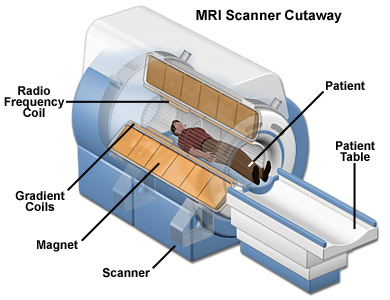
\includegraphics[width=.5\linewidth]{images/mri-scanner.jpg}
    \caption{\textbf{Schematic illustration} of construction of a cylindrical MRI scanner. Source:~\cite{coyne_mri_2020}.}
    \label{fig:mri_schematic}
\end{figure}

\subsection{Macroscopic Magnetization}
The purpose of the superconductive coils is to align the magnetic moment of protons with the direction of the magnetic field. This direction (also corresponding to the head-to-foot direction) is usually referred to as longitudinal direction or z direction, and the plane perpendicular to this direction is called the transverse plane or the x-y plane. This alignment of the magnetic moment of the protons leads to two configurations: protons with their magnetic moment pointing to the same direction as the static magnetic field, and other protons having their magnetic moment with opposite direction. Without the static field, the randomly oriented spins cancel out each other, as they also do in the aligned case, when the number of protons oriented to the two directions are equal. But in real systems, a slight excess of the protons aligned with the static magnetic field always produces a net magnetization with the same direction as the external magnetic field (see fig.\ref{fig:net_magnetization}).

The ratio of the number of protons in these two groups are described by the Fermi-Dirac statistics. In strong and static magnetic field at room temperature, the Fermi-Dirac distribution reduces to Boltzmann distribution resulting the following formula:
\[N_+ = N \cdot \frac{e^{E_+ / (k_B T)}}{e^{E_+ / (k_B T)} + e^{E_- / (k_B T)}} \text{ and } N_- = N \cdot \frac{e^{E_- / (k_B T)}}{e^{E_+ / (k_B T)} + e^{E_- / (k_B T)}},\]
where $N$ is the total number of protons, $N_+$ and $N_-$ are the numbers of protons pointing to the same and opposite direction as the static magnetic field, $E_+$ and $E_-$ are their respective energy levels, $k_B$ is the Boltzmann-constant, and $T$ is the temperature. In this case neighboring energy levels are equidistant with the difference in the secondary spin quantum number of $\Delta m = \pm 1$ and the energy difference of $\nabla E = \gamma \hbar B_0$, where $\gamma$ is an empirical constant called gyromagnetic ratio (equals to $42.575 \cdot 2\pi$\SI{}{\mega\hertz/\tesla} in case of protons), $\hbar$ is the reduced Planck constant, and $B_0$ is the static external magnetic field. The ratio of Boltzmann distributions for two states a spin \textonehalf nucleus is known as the Boltzmann factor:
\[f(E) = e^{-\frac{\gamma \hbar B_0}{k_B T}}.\]
Using this factor, the ratio of unpaired protons (these protons give the net magnetization) divided by the number of all protons is given by
\[\frac{N_+ - N_-}{N_+ + N_-} = \frac{\gamma \hbar B_0}{2 k_B T}.\]
This ratio at room temperature in a static field with a couple teslas is a tiny number (in the order of \num{1e-6} multiplied by $B_0$), so that explains why do MRI machines need such a strong electromagnets. (Note that this ratio also can be increased by increasing the temperature, but it is not feasible for human imaging.)

\begin{figure}[thb]
    \centering
    \begin{minipage}{.52\textwidth}
        \centering
        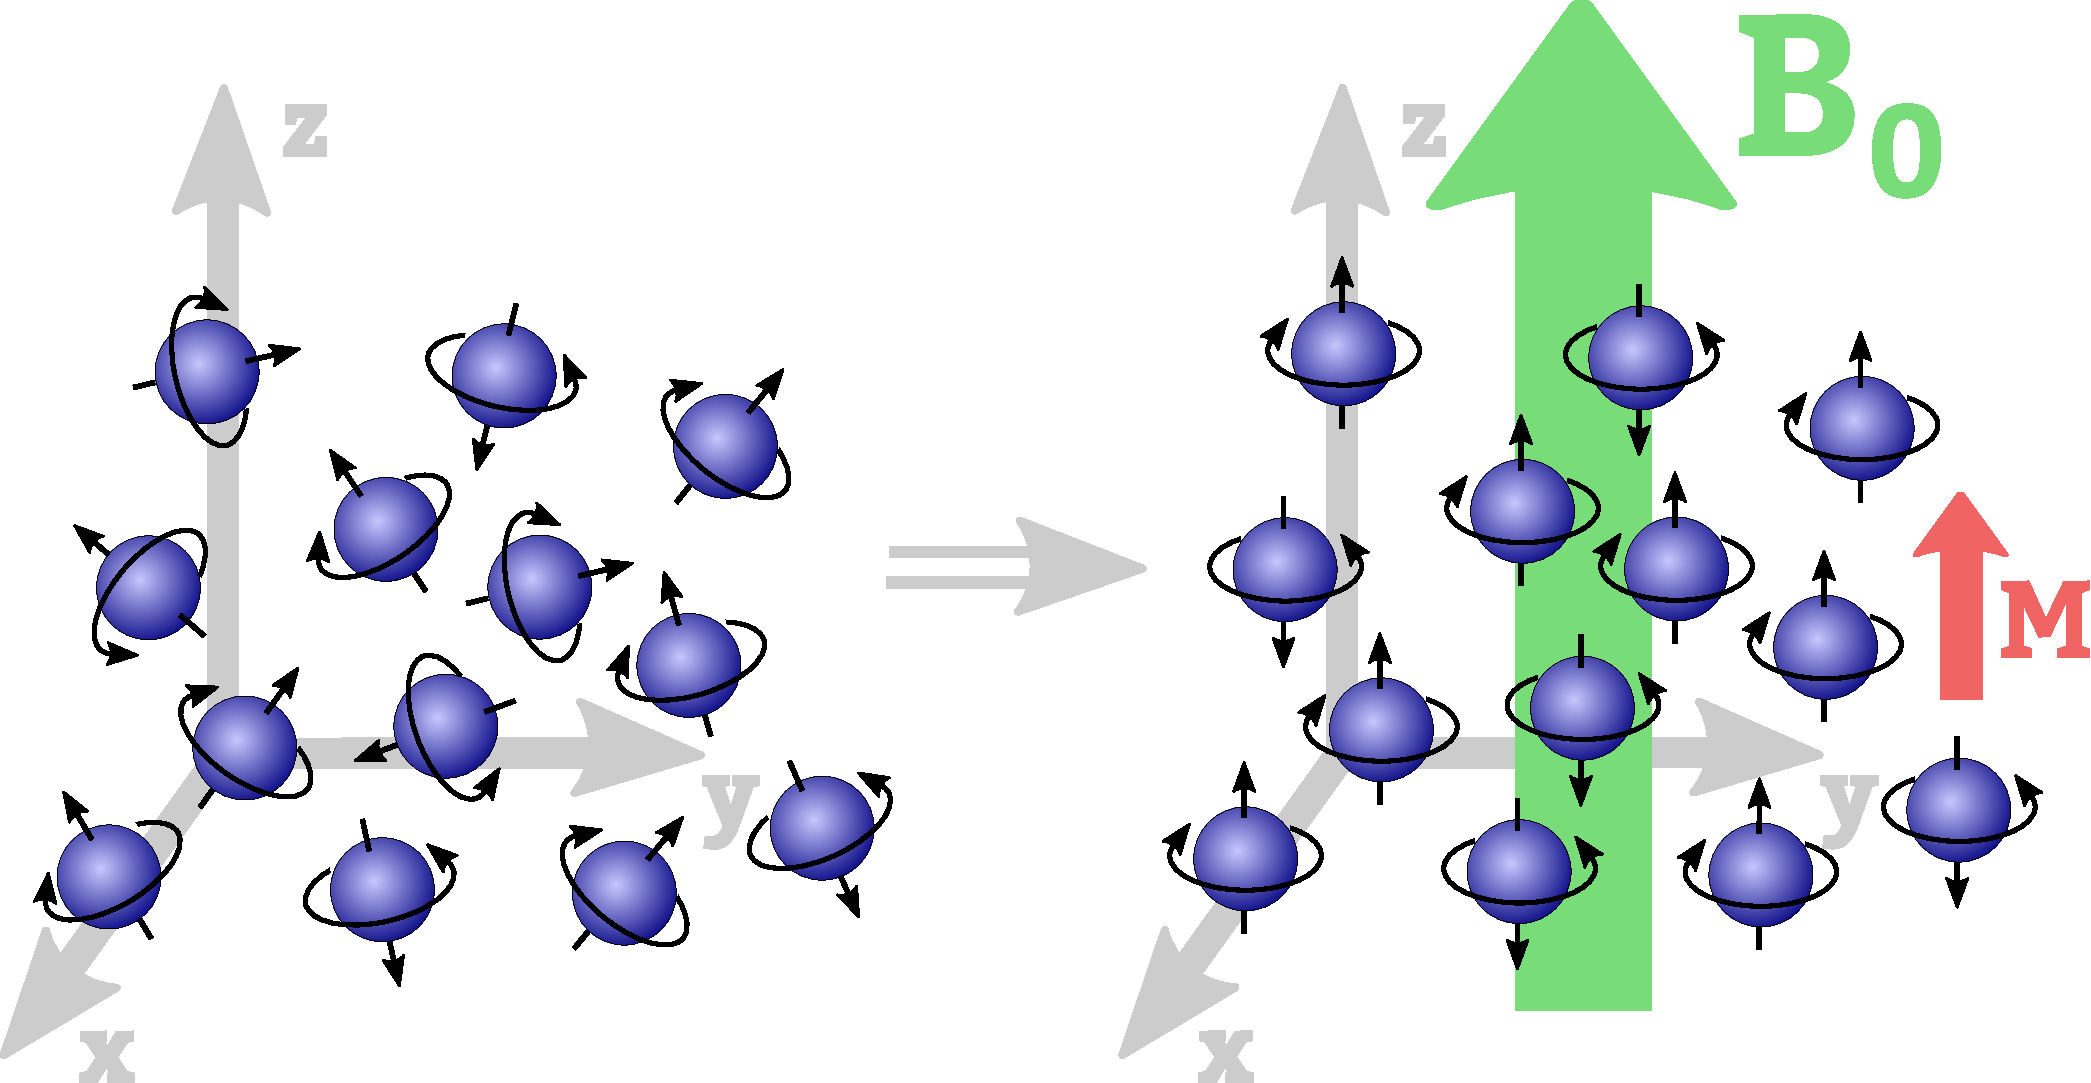
\includegraphics[width=0.8\linewidth]{images/net_magnetization.pdf}
        \caption{\textbf{Effect of strong external magnetic field ($B_0$):} Spins of protons get aligned with the field in either parallel or anti-paralellel direction producing a net magnetization ($M$) parallel with the external field.}
        \label{fig:net_magnetization}
    \end{minipage}%
    \hspace{0.03\textwidth}
    \begin{minipage}{0.44\textwidth}
        \centering
        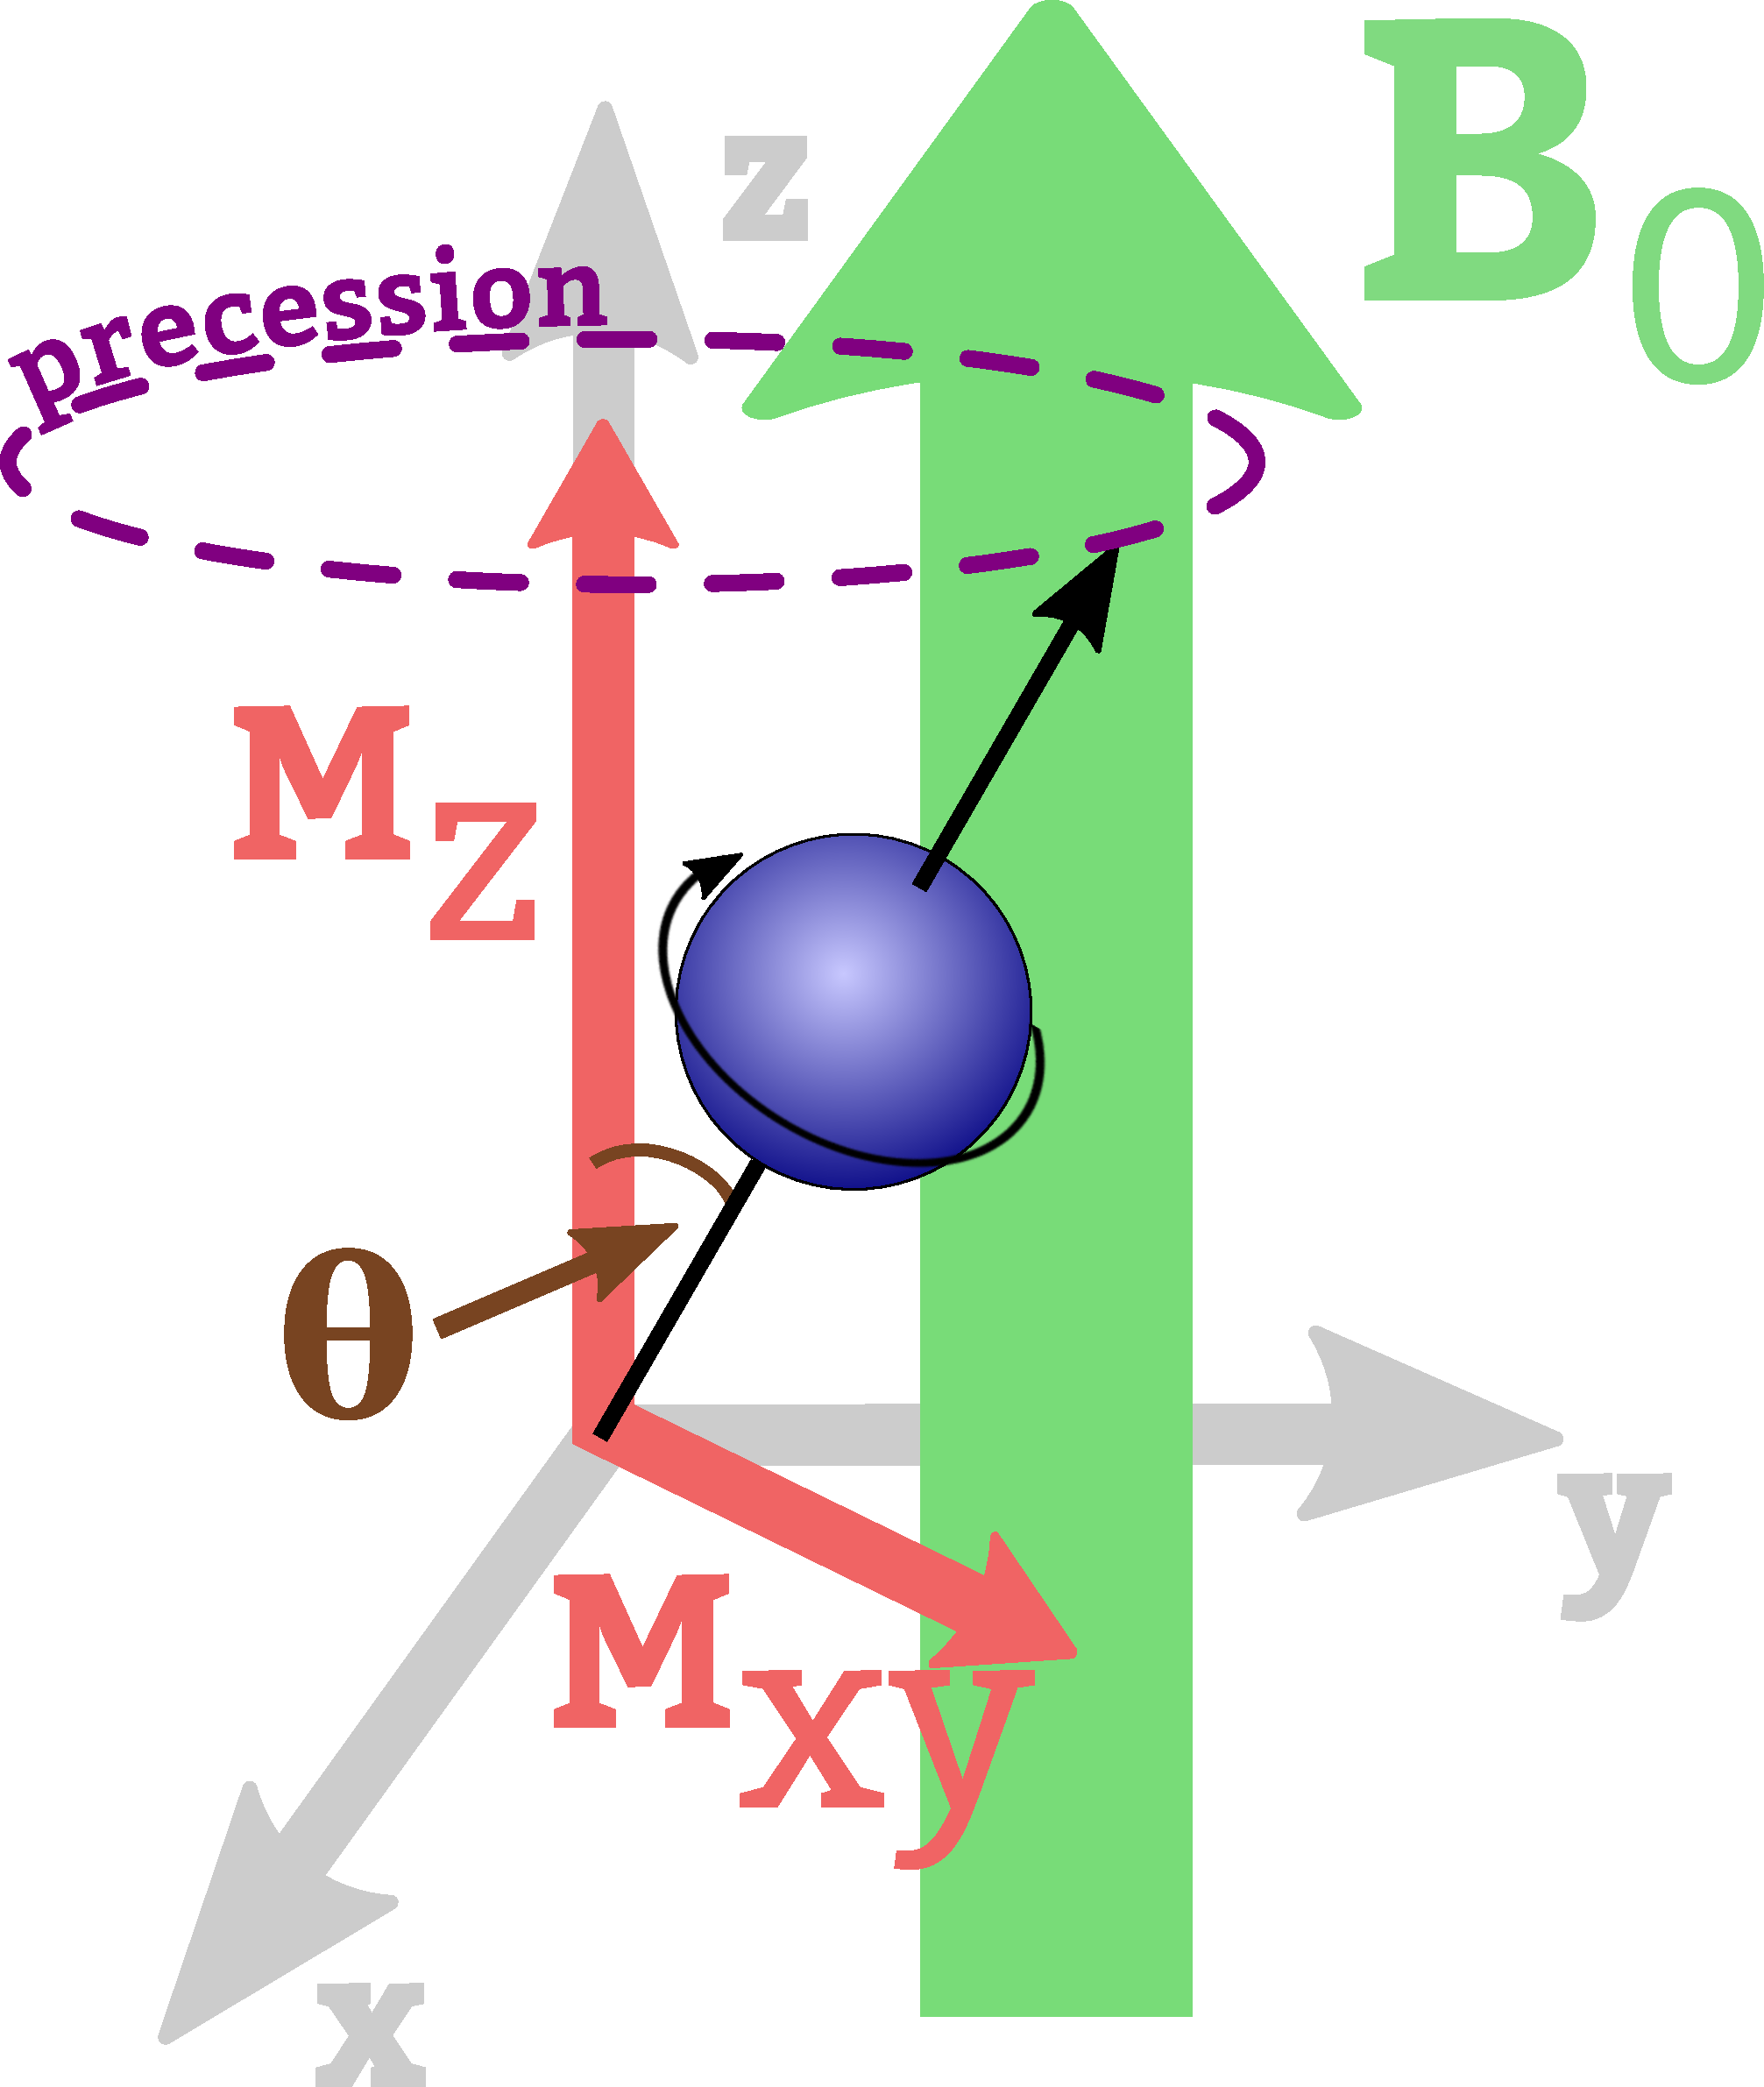
\includegraphics[width=0.4\linewidth]{images/precession.pdf}
        \caption{\textbf{Precession of protons.} As a result of RF excitation pulse, the magnetic momentum of protons deviates from the longitudinal direction and starts to precess due to its angular moment.}
        \label{fig:precession}
    \end{minipage}
\end{figure}

\subsection{Precession}
In equilibrium when all protons are aligned with the external magnetic field, the longitudinal component of net magnetization is maximal and the component in the transverse plane is zero. However, with the aid of an electromagnetic excitation in the transverse plane emitted by the RF coils, it is possible to rotate the vector of net magnetization into the transverse plane. The key factor in this process is to tune the frequency of the excitation to match the so called precessional frequency of the protons given by the Larmor equation:
\[\omega = \gamma B_0.\]
The name \textit{precessional frequency} comes from the phenomenon that the magnetic moment of protons start to precess around the longitudinal axis (which, again, is the direction of static external magnetic field) due to its intrinsic angular momentum. When the frequency of the excitation matches the precessional frequency of the proton (which happens to be in the radio frequency range, hence the name of RF coils), then resonance occurs and the angle of net magnetization gets tilted (illustrated by fig.~\ref{fig:precession}), otherwise the electromagnetic field has little to no effect of the net magnetization. An RF excitation of a duration $\tau$ causes rotation of the magnetization by an angle $\theta$, which is called the flip angle, defined by
\[\theta = \gamma \int_0^\tau B_1(t) dt = \gamma \tau B_1,\]
where $B_1$ is the magnetization of RF excitation, and it is assumed to be constant over time window of excitation with length $\tau$.

As a result of the precession, the net magnetic flux changes in the RF coils (these coils used for both emitting and receiving RF signals) inducing an electromotive force $U_{ind}$ that can be calculated by Faraday's law of induction:
\[U_{ind} = -\frac{d\Phi}{dt}.\]
Projecting the precessing movement (with the Larmor frequency $\omega$) of the net magnetization to transversal plan, we get a sinusoidal change in flux that results in the following formula:
\[U_{ind} \sim sin(\theta)\, \omega\, cos(\omega t) = sin(\theta)\, \gamma\, B_0\, cos(\gamma\, B_0\ t).\]
While this formula is not an exact model that fits the current measured in the RF coils, but it captures three important aspects of the resulted electric signal:
\begin{itemize}
    \item It is a sinusoidal signal with a frequency depending only on a constant specific to protons and the external magnetic field.
    \item The amplitude of that signal depends on the flip angle induced by an RF excitation.
    \item And it is also dependent on the external magnetic field (yet another reason why MRI machines need very strong electromagnets).
\end{itemize}

\subsection{Relaxation}
For a more accurate model, one should consider that as the protons emit RF signal due to their precessing magnetic moment, they lose the energy of the excitation and they slowly return to the low energy state; i.e., to the state where the magnetic moment of protons are aligned along the longitudinal axis, and where the net magnetization points to the same direction as the external field. Assuming that the excitation resulted in a perpendicular flip angle, the longitudinal component of magnetization is characterized by the exponential formula
\[M_z = M_0 (1 - e^{-t/T_1}),\]
where $M_0$ is the amplitude of magnetization in the equilibrium and is often called Boltzmann magnetization, and $T_1$ time constant is a property of the protons dependent on the tissue where they are located. The name of this process is $T_1$ relaxation.

\begin{figure}[thb]
    \centering
    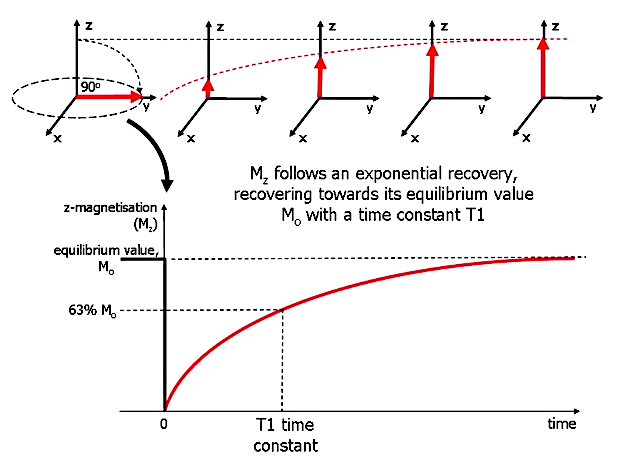
\includegraphics[width=0.8\linewidth]{images/T1_relaxation.png}
    \caption{\textbf{$T_1$ relaxation after a \SI{90}{\degree} RF excitation.} By the end of the pulse, the magnetization rotated from the z-direction to the x-y plane; therefore, the longitudinal component is reduced to zero, and gradually it returns to the equilibrium. Source:~\cite{ridgway_cardiovascular_2010}.}
    \label{fig:T1_relaxation}
\end{figure}

Furthermore, the net magnetization is also affected by another relaxation process called $T_2$ relaxation. The phenomenon causing this relaxation is called \textit{dephasing}, and the name comes from the fact that when excitation is applied to protons in the equilibrium, they will precess in the same phase, but soon they lose this synchronization. This desynchronization is due to the slight inhomogeneity of the static external field caused by four factors: spin-spin interactions (quantum mechanical interactions with the nearby protons), magnetic field inhomogeneities (hardware limitations), magnetic susceptibility (slight magnetization of molecules within the measured part of the body), and chemical shift effects (shielding effect of the electron cloud of molecules incorporating the hydrogen atoms). The slightly different $B_0$ value makes the Larmor frequency different, and that results in the desynchronization of phase. The outcome of this process is that the transversal component of the net magnetization decays exponentially to zero. The speed of decay is characterized by the $T_2^*$ time constant:
\[M_{xy} = M_1\,e^{-t/T_2^*},\]
where $M_1$ is the initial amplitude of net magnetization in the beginning of the $T_2$ relaxation process. For illustration of this process, see fig.~\ref{fig:T1_relaxation}. The resultant decaying signal is known as the Free Induction Decay (FID). Using, however, the later described \textit{spin-echo} acquisition protocol, the last three inhomogeneity-causing factors can be cancelled out leading to a slightly different time constant denoted by $T_2$.

\begin{figure}[thb]
    \centering
    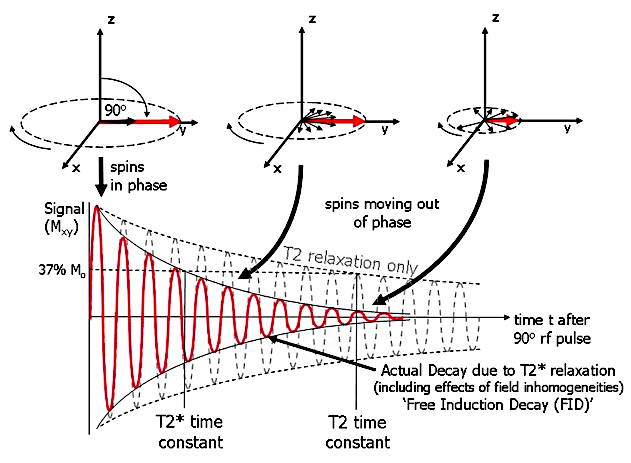
\includegraphics[width=0.8\linewidth]{images/T2_relaxation.png}
    \caption{\textbf{$T_2$ relaxation process.} Right after the RF pulse, thre precession of all protons are in the same phase, but they quickly desynchronize due to magnetic field inhomogeneities. The plot in the second row depicts the strength of current induced in the RF coils that corresponds to the projection of the x-y component ($M_{xy}$) of the net magnetization along the direction perpendicular to the surface of the coil. And as a result of the $T_2$ relaxation, the amplitude of this sinusoidal curve exponentially decays. The resultant decaying signal is known as the Free Induction Decay (FID). Source:~\cite{ridgway_cardiovascular_2010}.}
    \label{fig:T2_relaxation}
\end{figure}

\section{Concepts of MR Imaging}

In that section, the most important concepts of MR imaging are summarized, clarifying the vocabulary used in the later chapters, based on~\cite{nishimura_principles_1996, pooley_fundamental_2005}.

\subsection{MRI Sequences}
Since the advent of MRI, numerous methods were developed and are used in today's medicine. And while they are all measure somehow the $T_1$ and $T_2$ constants at different location, the produced image is quite different, making them fit different use cases. These methods are called MRI sequences and they mostly differ in the a particular setting of RF pulses and the gradients in the static magnetic field, resulting in a particular image appearance. The most commonly used group of MRI sequences is the \textit{spin echo}~\cite{hahn_spin_1950}. In accordance with the two types of relaxation, sequences in that group have two main parameters: $TR$ (Time of Repetition) and $TE$ (Time of Echo). These parameters have a crucial role timing the recording of current in the RF coils when the difference between the amplitude of the RF signal emitted by the excited protons is maximal because this difference makes it possible later to distinguish different tissues.

The $TR$ parameter is connected to the $T_1$ value, as it determines the time between two excitation pulses. Having a larger $TR$ value allows protons to get better aligned with the external magnetic field before the next excitation, which results in a higher initial value for $M_{xy}$, leading to a stronger current in the detector coils, but it also makes the entire measurement longer. On the other hand, $TE$ determines the delay between the peak of the RF pulse and the peak of the echo. That echo is a temporary rephasing of spins caused by a second, \SI{180}{\degree} RF pulse emitted at $t = TE/2$. That pulse inverts spins, and therefore it makes spins with slower Larmor frequency, which lagged behind the faster ones previously, be ahead of the others in phase. At the time when faster precessing protons catch up, the transversal magnetization exhibits an echo peak (see~\ref{fig:spin_echo}). As stated earlier, an important advantage of spin echo technique is that three factors of magnetic inhomogeneity is cancelled out by the inversion as these factors are constant over time, while spin-spin interactions are random interactions between protons that cause random local changes in the magnetic fields experienced by the protons.

\begin{figure}[thb]
    \centering
    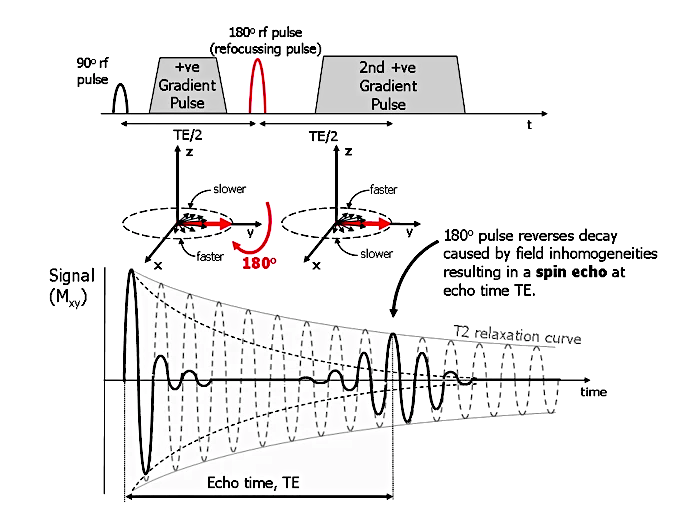
\includegraphics[width=0.8\linewidth]{images/spin_echo.png}
    \caption{\textbf{Process of spin echo sequence.} The echo is a temporary rephasing of spins caused by a second, \SI{180}{\degree} RF pulse emitted at $t = TE/2$. That pulse inverts spins, and therefore it makes spins with slower Larmor frequency, which lagged behind the faster ones previously, be ahead of the others in phase. At the time when faster precessing protons catch up, the transversal magnetization exhibits an echo peak. Source:~\cite{ridgway_cardiovascular_2010}.}
    \label{fig:spin_echo}
\end{figure}

Before moving forward, an important thing to note that the $T_1$ relaxation is much slower than the $T_2$ relaxation ($T_1$ relaxation takes hundreds of milliseconds up to a few seconds while $T_2$ rarely exceeds \SI{200}{\milli\second}. As a result, the acquisition time is mostly dominated by waiting for the $T_1$ relaxation, and therefore short $TR$ values are favorable when fast imaging is needed. Also, the different time-scale of $T_1$ and $T_2$ relaxation opens a range of possibilities to make acquisition process faster or more effective.

Based on the choice of $TR$ and $TE$ values, we can talk about three types of spin echo sequences: $T_1$ weighted sequence has intermediate $TR$ value in the magnitude of $T_1$ producing maximal T1 weighting (at this point, the difference caused by different $T_1$ value between the amplitude of signals coming from different tissues are maximal) and short $TE$ value magnitudes smaller than $T_2$ producing minimal T2 weighting (there is not enough time to have significant difference between decay curves with different $T_2$). To the contrary, T2-weighted images have a long $TE$ (maximizing the difference in $T_2$ relaxation) and long $TR$ (reducing the weight of $T_1$ relaxation). And the third type, called proton density (PD) weighting, uses short $TE$ and long $TE$, so that the pixel intensities on the resulted image will reflect only the density of protons (that also differs between tissues), and the $T_1$ and $T_2$ values have little effect on it.

\begin{figure}[thb]
    \centering
    \begin{minipage}[t]{.28\textwidth}
        \centering
        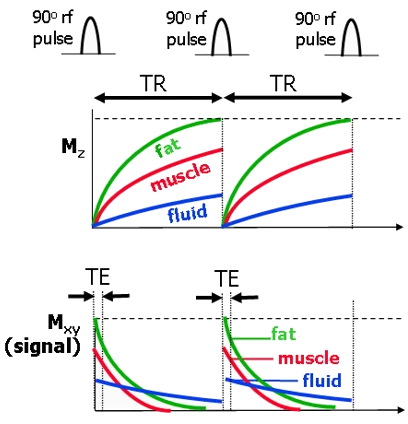
\includegraphics[width=.8\linewidth]{images/T1_weighted.png}
        \caption{\textbf{$T_1$ weighted sequence.} Choosing the $TR$ value to be relatively short, and $TE$ to be relatively short, the difference due to the variation of $T_1$ value over tissues would dominate over differences caused by different $T_2$ value. Source: Adapted from~\cite{ridgway_cardiovascular_2010}.}
        \label{fig:T1_weighted}
    \end{minipage}%
    \hspace{0.02\textwidth}
    \begin{minipage}[t]{.28\textwidth}
        \centering
        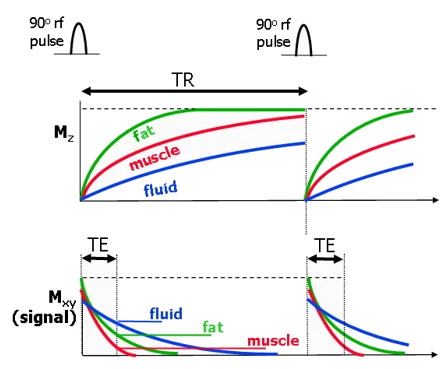
\includegraphics[width=\linewidth]{images/T2_weighted.png}
        \caption{\textbf{$T_2$ weighted sequence.} Choosing both $TR$ and $TE$ values to be relatively long, the difference due to the variation of $T_2$ would dominate over differences caused by different $T_1$ value. Source: Adapted from~\cite{ridgway_cardiovascular_2010}.}
        \label{fig:T2_weighted}
    \end{minipage}%
    \hspace{0.02\textwidth}
    \begin{minipage}[t]{0.34\textwidth}
        \centering
        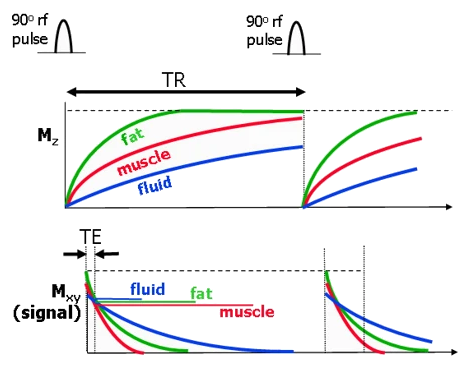
\includegraphics[width=.85\linewidth]{images/PD_weighted.png}
        \caption{\textbf{Proton density (PD) weighted sequence.} Choosing the $TR$ value to be relatively long, and $TE$ to be relatively short, the difference due to the variation of both $T_1$ and $T_2$ values are minimized, and hence mostly the density of protons would determine signal strength. Source: Adapted from~\cite{ridgway_cardiovascular_2010}.}
        \label{fig:PD_weighted}
    \end{minipage}
\end{figure}

Two common variant of spin echo are multiecho spin-echo, and turbo spin-echo. The multiecho spin-echo pulse sequence utilizes multiple \SI{180}{\degree} RF pulses to induce multiple echo peaks each with a different $TE$, forming multiple images of the same object with different weighting ranging from PD-weighting to $T_2$-weighting. This method exploits the fact that $T_1$ is much larger than $T_1$, thus multiple echos can be performed without drastically changing the acquisition time. Similarly, turbo spin-echo sequences consist of multiple echo-generating \SI{180}{\degree} pulses, but in this case only one image is formed speeding up the imaging by gathering information about multiple positions in each cycle.

The other large group of sequences is the gradient echo sequence~\cite{winkler_characteristics_1988}. That type of sequences differs from echo-spin that the flip angle of initial RF pulse is less than \SI{90}{\degree} (e.g., \SI{20}{\degree} or \SI{30}{\degree}) and there is no \SI{180}{\degree} secondary pulse, instead it induces an echo by the spacial gradients explained later. Hence this method is able to perform the measurement much faster as $T_1$ relaxation reaches near-equilibrium state much earlier.

Beyond these sequence types, several other commonly used variants exist, which will not be discussed here, such as the inversion recovery sequences~\cite{dwyer_short-ti_1988, fleckenstein_fast_1991, ashgriz_flair_1991, bedell_implementation_1998}, diffusion-weighted sequences~\cite{moseley_diffusion-weighted_1990, bammer_basic_2003}, perfusion weighted sequences~\cite{rosen_perfusion_1990, detre_perfusion_1992, barbier_methodology_2001}, BOLD-contrast images for functional MRI (fMRI)~\cite{ogawa_brain_1990, kwong_dynamic_1992}.

\subsection{Spatial Encoding}
The core concept that allowed the extension of NRM (which is based on the same principles described above) to MRI, is the spatial encoding. This technique, proposed by Paul Lauterbur, allows for the localization of RF emitting protons or, more precisely, the localization of an \textit{ensemble} of RF emitting protons within a small volume called voxels (note that the size and the shape of these voxels are defined by the configuration of MRI machine for the given acquisition). Specifically, the problem with static magnetic field is that, even though the net magnetization varies over the measured object based on the type of the tissue, the RF pulse excites the entire volume of the measured object, and therefore the induced signal of each voxel sum up making it impossible to separate them based on their position. In contrast, generating a secondary magnetic field with a gradient along a specific direction makes the Larmor frequency dependent on the position along that direction. That dependence can be exploited multiple ways allowing exact localization along all three dimensions. A possible (and quite common) way to do this is the following:
\begin{enumerate}
    \item Producing a gradient along the z-direction during the RF excitation permits the selection of a slice perpendicular to the z-axis by tuning the RF pulse to the frequency specific to the given slice because this pulse excites then only protons in the selected slice. In reality, however, not a single frequency used but rather a band of frequencies whose width matches the bandwidth of resonance frequencies of spins in the slice of interest. This approximately rectangular band of excitation frequencies is realized in time domain by a pulse of a shape similar to the sinc function.
    \item Application of another gradient along the y-direction between the RF excitation and the readout of induced current causes a gradual de-synchronization of phase along the y-axis because protons experiencing higher external field will have a higher Larmor frequency as well. Therefore, the position along y-direction becomes \textit{phase-encoded}.
    \item During the time window of readout, another gradient along the x-direction can be used to separate signal sources along that dimension by the difference in their frequency. This type of spacial encoding is called \textit{frequency encoding}.
\end{enumerate}
These steps are visually explained on fig.~\ref{fig:slice_selection} and~\ref{fig:phase_and_freq_encoding}.

\begin{figure}[thb]
    \centering
    \begin{minipage}{.43\textwidth}
        \centering
        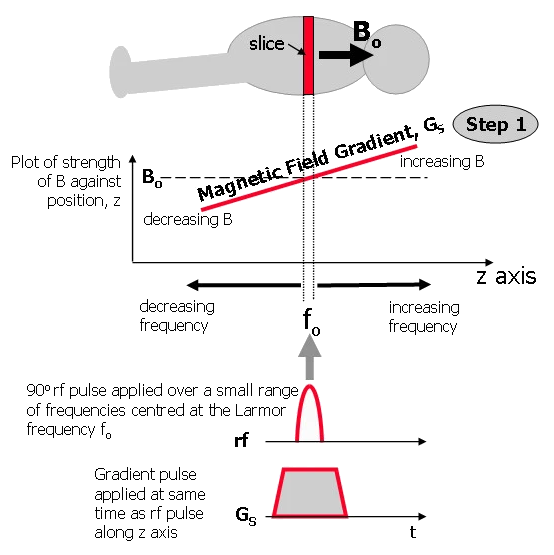
\includegraphics[width=\linewidth]{images/slice_selection.png}
        \caption{\textbf{Mechanism of slice selection.} Producing a gradient along the z-direction during the RF excitation permits the selection of a slice perpendicular to the z-axis by tuning the RF pulse to cover the frequency range specific to the given slice with given thickness because this pulse excites then only protons in this slice. Source:~\cite{ridgway_cardiovascular_2010}.}
        \label{fig:slice_selection}
    \end{minipage}%
    \hspace{0.03\textwidth}
    \begin{minipage}{0.53\textwidth}
        \centering
        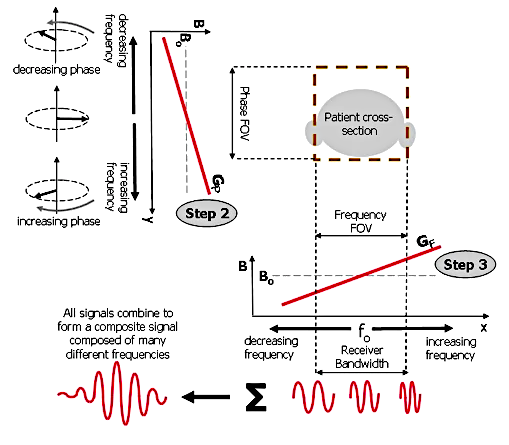
\includegraphics[width=\linewidth]{images/phase_and_freq_encoding.png}
        \caption{\textbf{Process of phase and frequency encoding.} First, a gradient along the y-direction between the RF excitation and the readout causes a gradual de-synchronization of phase along the y-axis because protons experiencing higher external field will have a higher Larmor frequency. Second, a gradient along the x-direction can be used to separate signal sources along that dimension by the difference in their frequency. Source:~\cite{ridgway_cardiovascular_2010}.}
        \label{fig:phase_and_freq_encoding}
    \end{minipage}
\end{figure}

Decoding the spatial information becomes feasible then using the famous Bloch equation:
\[\frac{d\mathbf{M}}{dt} = \mathbf{M} \times \boldsymbol{\gamma} \mathbf{B} - \frac{M_x\mathbf{i} + M_y\mathbf{j}}{T_2} - \frac{(M_z - M_0)\mathbf{k}}{T_1}.\]
Knowing that the transversal component of the net magnetization (that is, the measured component) is non-zero only a selected slice and is dependent on the position within the slice assuming the excitation strategy above, a convenient formulation is to use a complex-valued function to denote the amplitude of the signal generated at position $(x,y)$ by $m(x,y) = m_x(x,y) + m_y(x,y)$, where $m_x(x,y)$ and $m_y(x,y)$ is the amplitude realized in a coil perpendicular to x-axis and y-axis, respectively. As a result of the phase-encoding, the phase of a spin at position $y$ along y-axis is given by $\omega_0 t_y + \gamma G_y t_y y,$ where $\omega_0$ is the base Larmor frequency of the selected slice, $t_y$ denotes the width of time window of phase-encoding, and $G_y$ corresponds to the slope of the linear gradient applied along the y-direction. Because $m(x,y)$ is a complex-valued function representing the magnetization in both the x and y-direction, the distribution $m(x,y)$ gets weighted by a complex exponential corresponding to the spatial frequency $\gamma/2\pi)G_y t_y$: $m(x,y)exp(-i\gamma G_y t_y y$. 

Similarly, the shift in the frequency of precession during the readout characterized by $\gamma G_x x$ adds another weighting term to $m(x,y)$. Solving the Bloch equation for this configuration results in the following formula:
\[s(t) = \int_x \int_y m(x,y) e^{-i\gamma G_x x t} e^{-i\gamma G_y y t_y} dx dy,\]
where $s$ is the amplitude of signal to be measured, $t_y$ (length of time window for phase-encoding) is a fixed number and $t$ is a running variable. Having a look at the formula, one can immediately see that it is the 2-dimensional Fourier transform of $m(x,y)$ corresponding to the coordinate $((\gamma/2\pi)G_x t, (\gamma/2\pi)G_y t_y)$ in the Fourier space. Due to the discrete nature of this the acquisition process, the MRI machines can evaluate the Fourier space in discrete positions, that is, the collected data is the \textit{discrete Fourier transform} (DFT) of the object. Consequently, the space of measurements is usually referred to as k-space. This connection between the measured signal and Fourier transformation is beneficial in many aspects, as it will be apparent in the next sections.

\subsection{Sampling Trajectories}
The effect of the spatial encoding schema discussed above is that the k-space points can only be measured sequentially. Combined with the necessity of waiting for the $T_1$ relaxation (that tends to be in the timescale of  \SIrange{250}{1500}{\milli\second} at \SI{3}{T}, and somewhat shorter for \SI{1.5}{T}~\cite{gold_musculoskeletal_2004,bojorquez_what_2017,stanisz_t1_nodate}), it leads to the most important limitation of MR imaging: the acquisition is quite slow. While it is inconvenient for the patient to stay inside the narrow scanner bore (especially for claustrophobic patients), the more important issue is that the longer is the acquisition the more motion artifacts are introduced to the image. The type of such involuntary motions include bulk motion (e.g., coughing, change body position), respiratory motion, cardiac motion, and motion of other organs like blood vessels or parts of the gastrointestinal tract. Although some of them can be reduced by a large extent, for example, by asking patient to pay attention to remain still or to hold breath for a \SIrange{10}{20}{\second} long measurement, others are out of control. Reducing the k-space points, however, lead to various aliasing effects according to Nyquist-Shannon sampling theorem that might blur clinically relevant features or introduce misleading artifacts. Therefore, radiologists always seek to find an optimal compromise between the number of measured k-space points and the amount of motion artifacts introduced.

One important aspect of dealing with that problem is determining which points are to be measured. Due to hardware limitations and because too rapidly changing electromagnetic field would overheat the measured tissues, arbitrary positioning in k-space is not feasible, and thus the order of measurement points are also a key aspects of the process. These constrains introduces the necessity of well-defined geometries describing the location and the order of measured k-space coordinates, called sampling trajectories.

The traditional way of acquiring K-space data is through Cartesian trajectories. The concept of these trajectories is that equally spaced grid-points are selected in the slice or volume to be measured, and these points are evaluated systematically; for instance, row-by-row, zig-zag, or spirally. The main benefit of this method that a simple and fast reconstruction is possible via fast Fourier transform (FFT). Nevertheless, this method fails to exploit a very important feature of natural images in general: the energy tends to be concentrated in the center of the Fourier space; that is to say, the coefficients of lower frequencies have usually large magnitudes, and points further from the center have mostly a near-zero value. The significance of this observation is perfectly demonstrated by the success of the modern image and video compression algorithms making use of this uneven distribution, for instance, JPEG~\cite{wallace_jpeg_1992} and H.26x video compression family~\cite{farooq_study_2017} (on which most modern audio video file formats are based on, like mp3 and mp4). Hence, multiple non-equidistant sampling trajectories are also used in practice. Such trajectories are radial~\cite{rasche_continuous_1995}, spiral~\cite{blum_fast_1987}, concentric rings~\cite{wu_mri_2008}, and 3D cones trajectories~\cite{gurney_design_2006}, just to name a few. A couple 3-dimensional trajectories are depicted in fig.~\ref{fig:trajectories}.

\begin{figure}[tb]
    \centering
    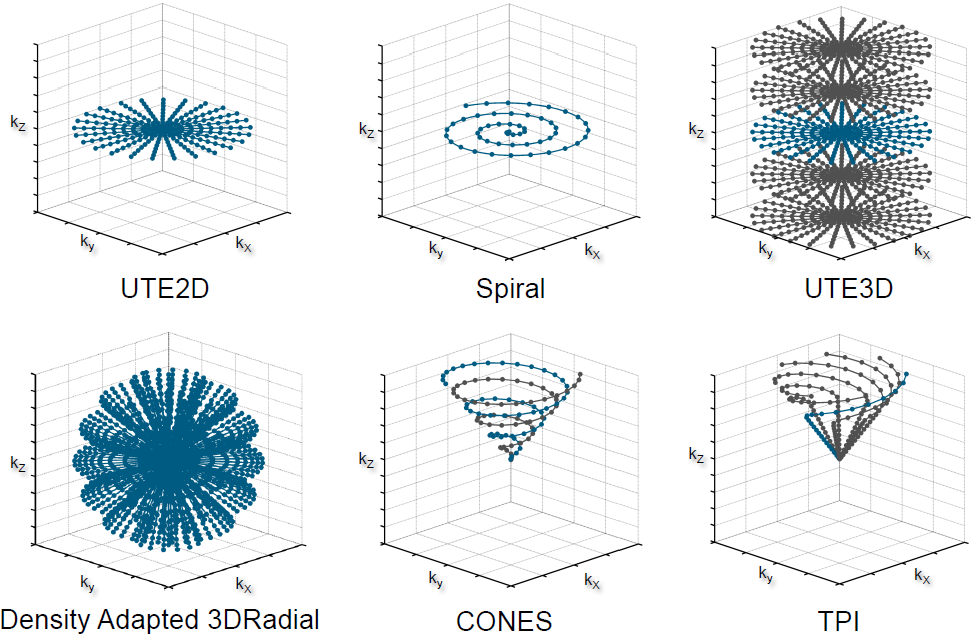
\includegraphics[width=0.8\linewidth]{images/trajectories.png}
    \caption{\textbf{A few example for 3D trajectories.} Source:~\cite{noauthor_forschungszentrum_nodate}}
    \label{fig:trajectories}
\end{figure}

\subsection{Accelerated MRI}\label{section:accelerated}
For a deeper understanding of accelerating methods, one needs to get familiarized with the concept of field of view and its connection to the bandwidth of RF excitation pulse. The term \textit{field of view} (FOV) refers to the area or volume over which an MR image is acquired, and often also to its size as well. Due to the discrete nature of digital systems, the FOV is also discretized representing it with a grid of equidistant points whose values in grid points can then be displayed as pixels on computer screens. The two main parameters of FOV are therefore its size and the pixel width. The size of FOV is proportional to the bandwidth of RF excitation and inverse proportional to the strength of the frequency encoding gradient. Thus, it makes increasing the RF bandwidth is beneficial for the image quality (although is comes with increased production costs as well), and it limits the strength of the frequency encoding gradient, even though stronger gradient would be advantageous to better separate tissues by their precessional frequencies. In contrast, the pixel size is determined by the size of range over which k-spaces samples are collected. In case of equidistant sampling in k-space over a square shaped FOV, the connection between these parameters can be expressed by simple equations:
\[\Delta k = 1 / FOV \text{ and } \Delta w = 1 / k_{FOV},\]
where $\Delta k$ is the distance between k-space points, $FOV$ refers to the size of the FOV, $\Delta w$ is the pixel width, and $k_{FOV}$ is defined as the range between the highest positive and largest negative spacial frequencies in k-space (i.e., $k_{FOV} = k_{max}^+ - k_{max}^- = 2 \cdot k_{max}$, if $k_{max}^+ = |k_{max}^-|$). For a visual example, please refer to fig.~\ref{fig:cartesian}.

\begin{figure}[htb]
    \centering
    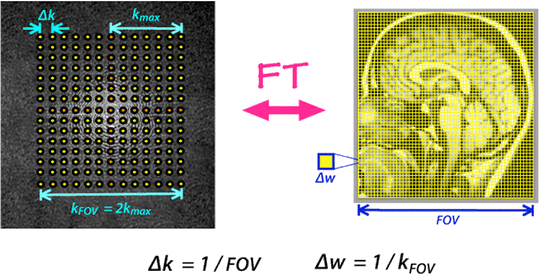
\includegraphics[width=0.6\textwidth]{images/cartesian.png}
    \caption{\textbf{Connection between FOV and k-space} in case of Cartesian sampling: The size of FOV is inversely proportional to the distance of k-space points, and the pixel size is determined by the size of range over which k-spaces samples are collected. Source:~\cite{noauthor_kspace_nodate}.}
    \label{fig:cartesian}
\end{figure}

Using these concepts, one can formulate many methods to accelerate acquisition. For instance, it is possible to evaluate only half of the k-space exploiting the underlying symmetry in the Fourier transform. This method is successful in maintaining a high resolution, albeit it come with the cost of reduced signal-to-noise ratio (SNR) because of the lack of the noise-cancelling effect of two-sided measurements. Another popular method is to avoid acquiring the periphery of k-space by limiting the range of the phase-encoding frequencies (which, in fact, are connected to $T_1$ relaxation that contributes the most to the acqisition time). The advantage of this method is that it produces a decent speed-up keeping the SNR relatively high, but undersampling the high frequencies have a blurring effect, and therefore the resolution goes down. Finally, it is also possible to reduce the size of the FOV leading to a rectangular shaped image (also by reducing the phase-encoding step). The speed-up here, however, also comes with a cost: the amount of noise unfortunately remains the same as in the case of the wider FOV, but now it is distributed over a smaller area, and consequently the SNR also goes down.

A similar, but more effective method is proposed to accelerate imaging using multiple independent RF coils are built around the measured object. That method is commonly referred to as parallel imaging (PI), and idea behind is that the placement and the sensitivity characteristics of the coils are known, therefore the amplitude of the measured signal can be used to assist the localization of the signal source. This additional information makes less phase-encoding steps sufficient for acquisition, and thus allows a potentially several-fold reduction in imaging time. For an illustrative example, see~\ref{fig:parallel_imaging}. While PI also have downsides, namely the increased production cost of PI-capable machines, the unavoidable reduction in SNR (because each coil has its own, independent noise that sums up at reconstruction), and the introduction of PI-specific artifacts that comes from the inaccurate estimation of the coils sensitivities over the FOV, and the uneven distribution of noise related to coil geometry, the effect of these drawbacks can be reduces by the increase of number of coils (albeit this further increases the production cost).

\begin{figure}[htb]
    \centering
    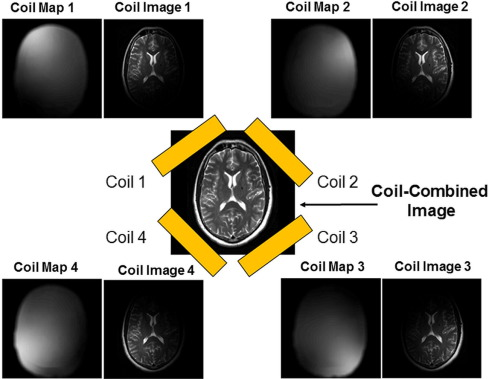
\includegraphics[width=0.8\linewidth]{images/parallel_imaging.jpg}
    \caption{\textbf{Illustrative example for parallel imaging technique.} Multiple independent RF coils are built around the measured object, and as the detection sensitivities of the coils are known, the amplitude of the measured signal can be used to assist the localization of the signal source. Source:~\cite{hamilton_recent_2017}}
    \label{fig:parallel_imaging}
\end{figure}

\subsection{Bottom Line}
Since the advent of MR imaging, an explosion of the amount of MRI concepts and technologies is witnessed by the scientific community during the last 3-4 decades. Although the quality of the images has undergone drastic improvement, placing MRI to the focus of today's diagnostic, the speed of evolution based on hardware-related innovations seems to slow down as the technology approaches its physical limits (e.g., the strength of the static magnetic field cannot be increased infinitely and the number of coils in PI is limited, for example, by the space available inside the machine). And while the acquisition time is significantly improved over time, but MRI is still considered to be a slow imaging technique, making dynamic imaging a challenging task. Hence, there is an increasing interest towards software solutions which can push further down the number of k-space points required to produce images with a quality sufficient for successful diagnosis.

\clearpage
\chapter{Mathematical Foundation}

The real power of the compressed sensing is that it has a firm mathematical background that provides guarantees for the solution under certain assumptions. In this chapter, we essay to describe the very basics of compressed sensing, and then give a quick overview of a few selected numerical methods, which will be later used in this work as building blocks of more complex algorithms. These descriptions follow the book~\cite{foucart_mathematical_2013} and are based on the lectures of the course titled \textit{Compressive Sampling} at Technical University of Munich by Alihan Kaplan.

\section{Elementary Definitions}

Although the reader might be to be familiar with the most of these definitions, for the sake of completeness and clarity of notation used in this work, we present here a list of definitions of elementary constructs, restricting ourselves to mere formulations with short remarks omitting further explanation.

\begin{tight_equations}

\begin{definition}[norm]
A non-negative function $\norm{\cdot}: X \rightarrow [0, \infty)$ is called a norm, if 
\begin{enumerate}[label=\alph*)]
    \item $\norm{\mathbf{x}} = 0$ if and only if $\mathbf{x} = \mathbf{0}$,
    \item $\norm{\lambda \mathbf{x}} = \Vert \lambda \Vert \norm{\mathbf{x}}$ for all scalars $\lambda$ and all vectors $\mathbf{x} \in X$, and
    \item $\norm{\mathbf{x} + \mathbf{y}} \le \norm{\mathbf{x}} + \norm{\mathbf{y}}$ for all vectors $\mathbf{x, y} \in X$.
\end{enumerate}
\end{definition}

\begin{remark}
$X$ denotes a vector space on which the norm is defined. In MRI setting, however, $\mathbb{C}^N$ is the default vector space for computations, and therefore, we also define the following constructs in this space.
\end{remark}

\begin{definition}[$\ell_p$-norms for vectors]
The $\ell_p$-norm on $\mathbb{C}^N$ is defined for $1 \le p < \infty$ as
\begin{equation}\label{eq:p-norm}
\norm{\mathbf{x}}_p = \left(\sum_{j=1}^n |x_j|^p\right)^{\frac{1}{p}},
\end{equation}
and for $p = \infty$ as
\[\norm{\mathbf{x}}_\infty = \max_{j \in [n]} | x_j |.\]
For $0 < p < 1$, (\ref{eq:p-norm}) defines a quasinorm, which means that from the definition of the norm a) and b) holds, but c) is replaced by the weaker quasitriangle inequality
\[\norm{\mathbf{x} + \mathbf{y}}_p \le C\left(\norm{\mathbf{x}}_p + \norm{\mathbf{y}}_p\right)\]
with $C = 2^{\frac{1}{2}-1}$.
\end{definition}

\begin{remark}
Figure~\ref{fig:balls} is showing 2-dimensional balls defined by $\ell_p$-norm with various $p$ values.
\end{remark}

\begin{figure}
    \centering
    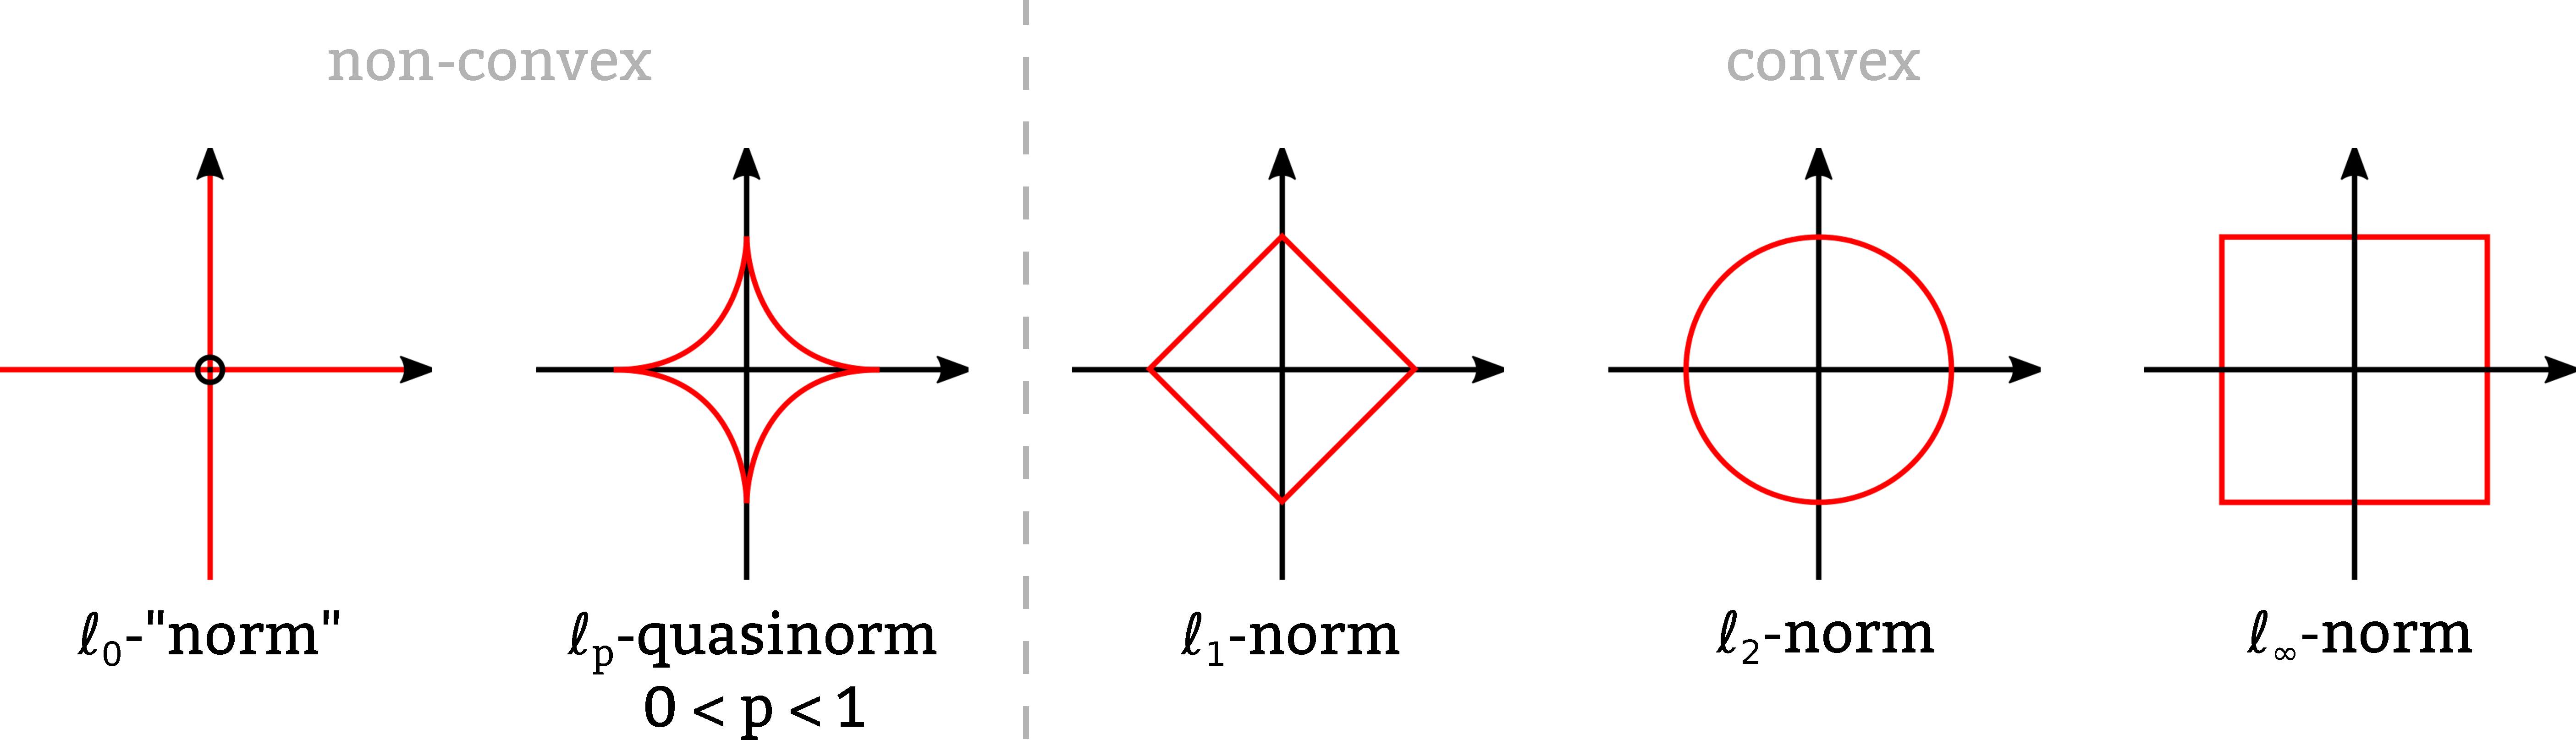
\includegraphics[width=\textwidth]{images/balls.pdf}
    \caption{\textbf{$\ell_p$ balls in 2D.}}
    \label{fig:balls}
\end{figure}

\begin{notation}
$[n]$ denotes the set of integers form $0$ to $n-1$.
\end{notation}

\begin{remark}
Using the schema above, it is impossible to have a proper norm for $p = 0$; nonetheless, is very common to define $\ell_0$-norm as the number of non-zero coordinates:
\[\norm{\mathbf{x}}_0 = \left| \left\{x_i \ne 0 : i \in [n]\right\}\right| \text{ where } \mathbf{x} \in \mathbb{C}^N.\]
Following this convention, $\norm{\cdot}_0$ always refers to that formulation in this work.
\end{remark}

\begin{definition}
The Frobenius norm on $\mathbb{C}^{m \times n}$ is defined as
\[\norm{\mathbf{A}}_F = \left(\sum_{i=1}^m\sum{j=1}{n}|a_{ij}|^2\right)^\frac{1}{2}.\]
\end{definition}

\begin{definition}[sparsity]
We call a vector $s$-sparse, if at most $s$ of its entries are non-zero; i.e. $\norm{\mathbf{x}}_0 \le s$.
\end{definition}

\begin{notation}
By $\Sigma_s^N$ we denote the set of all s-sparse vectors in $\mathbb{C}^N$; that is,
\[\Sigma_s^N = \left\{\mathbf{x} \in \mathbb{C}^N : \norm{\mathbf{x}}_0 \le s \right\}.\]
\end{notation}

%\begin{notation}
%The solution set $\left\{\mathbf{x} \in \mathbb{C}^N : \mathbf{Ax} = \mathbf{y}\right\}$ is denoted by $L_\mathbf{A}(\mathbf{y})$ for a given $\mathbf{A} \in \mathbb{C}^{m \times N}$.
%\end{notation}

%\begin{definition}[unique sparse solution]
%A vector $\mathbf{x}_* \in \mathbb{C}^N$ is the unique $s$-sparse solution of equation $\mathbf{Ax} = \mathbf{y}$ with $\mathbf{A} \in \mathbb{C}^{m \times N}$ and $\mathbf{y} \in \mathbb{C}^m$, if $L_\mathbf{A}(\mathbf{y}) \cap \Sigma_s^N = \{\mathbf{x}_*\}$, in other words, it is the only $s$-sparse vector satisfying the  linear system defined by $\mathbf{A}$ and $\mathbf{y}$.
%\end{definition}

\begin{definition}[kernel/null space]
The kernel/null space of a matrix $\mathbf{A} \in \mathbb{C}^{m \times N}$ is defined as
\[ker(\mathbf{A}) = \left\{\mathbf{x} \in \mathbb{C}^N : \mathbf{Ax} = \mathbf{0}\right\}.\]
\end{definition}

\begin{definition}[convex functions]
A function $f:\mathbb{C}^n \rightarrow \mathbb{R}$ is called convex, if for all $\mathbf{x}, \mathbf{y} \in \mathbb{C}^n $ and $t\in [0,1]$
\[f(t\mathbf{x} + (1-t)\mathbf{y}) \le t f(\mathbf{x}) + (1-t) f(\mathbf{y})\]
holds. Similarly, a function $f:\mathbb{C}^n  \rightarrow \mathbb{R}$ is called \textbf{strictly} convex, if for all $\mathbf{x} \ne \mathbf{y} \in \mathbb{C}^n $ and $t\in [0,1]$
\[f(t\mathbf{x} + (1-t)\mathbf{y}) < t f(\mathbf{x}) + (1-t) f(\mathbf{y})\]
holds.
\end{definition}

\begin{remark}
For $1 \le p < \infty$, the $\ell_p$-norms are strictly convex, and $\ell_p$-quasinorms for $0 < p < 1$ are always non-convex (see fig.~\ref{fig:balls}).
\end{remark}

\begin{remark}
A useful property of convex function is that all local minimizers are also global minimizers. Moreover, the minimizer of a \textit{strictly} convex function is unique, as well.
\end{remark}

\begin{definition}[Lipschitz-continuity]
A function $f:\mathbb{C}^n \rightarrow \mathbb{R}$ is said to be Lipschitz-continuous, if there exists a constant $L \in \mathbb{R}$ such that for all $\mathbf{x}, \mathbf{y} \in \mathbb{C}^n$
\[|f(\mathbf{x}) - f(\mathbf{y})| \le L \norm{\mathbf{x} - \mathbf{y}}_2\]
holds where $L$ is referred to as Lipschitz-constant.
\end{definition}

\begin{remark}
The set of Lipschitz-continuous functions is a superset of continuously differentiable functions.
\end{remark}

\begin{definition}[gradient and Hessian]
The gradient $\nabla f$ and the Hessian $\mathbf{H}_f$ of a function $f:\mathbb{C}^n \rightarrow \mathbb{R}$ at $\mathbf{x} \in \mathbb{C}^n$ is defined as follows:
\[\nabla f(\mathbf{x}) = \begin{bmatrix}
\frac{\partial}{\partial x_1} f(\mathbf{x}) \\ 
\frac{\partial}{\partial x_2} f(\mathbf{x}) \\ 
\vdots \\ 
\frac{\partial}{\partial x_n} f(\mathbf{x})
\end{bmatrix}, \mathbf{H}_f(\mathbf{x}) = \begin{bmatrix}
\frac{\partial^2}{\partial x_1^2} f(\mathbf{x}) & \frac{\partial^2}{\partial x_1 x_2} f(\mathbf{x}) & \ldots & \frac{\partial^2}{\partial x_1 x_n} f(\mathbf{x}) \\ 
\frac{\partial^2}{\partial x_2 x_1} f(\mathbf{x}) & \frac{\partial^2}{\partial x_2^2} f(\mathbf{x}) & \ldots & \frac{\partial^2}{\partial x_2 x_n} f(\mathbf{x}) \\ 
\vdots & \vdots & \ddots & \vdots \\ 
\frac{\partial^2}{\partial x_n x_1} f(\mathbf{x}) & \frac{\partial^2}{\partial x_n x_2} f(\mathbf{x}) & \ldots & \frac{\partial^2}{\partial x_n^n} f(\mathbf{x})
\end{bmatrix}.\]
\end{definition}

\begin{remark}
The geometric interpretation of gradient is that it is a vector in the tangent plane at a certain point on the surface defined by the function $f$, and this vector steepest direction where the value of $f$ increases the quickest. The Hessian, on the other hand, carries information about the curvature of the surface.
\end{remark}

\begin{definition}[order and rate of convergence]
An iterative method producing the sequence $\{\mathbf{x}_n\}$ is said to have a convergence of order $p$ to some $\mathbf{x}^*$ with respect to function $f:\mathbb{C}^n \rightarrow \mathbb{R}$, if there exists a number $\mu \in \mathbb{R}_+  \cup \{0\}$, called rate of convergence, such that
\[\lim_{k \rightarrow \infty} \frac{\norm{\mathbf{x}_{k+1} - \mathbf{x}^*}}{\norm{\mathbf{x}_{k} - \mathbf{x}^*}^p} < \mu.\]
\end{definition}

\begin{remark}
If $p = 1$, then the convergence is also referred to as a linear convergence. The special cases of linear convergence are \textit{superlinear} convergence when $\mu = 0$ and \textit{sublinear} convergence when $\mu > 0$. If $p=2$, then the convergence is called \textit{quadratic}.
\end{remark}

\begin{notation}
Besides the definition above, there are two other commonly used formulation to characterize the convergence speed using the big O notation. One way is expressing the time complexity by number of steps needed to approximate the solution under the maximal tolerated error $\epsilon$. For example, $ \mathcal{O}(\epsilon^-2)$ is a colloquial notation to express that the function will produce the approximation $\mathbf{x}_k$ such that 
\[|f(\mathbf{x}_{k}) - f(\mathbf{x}^*)| < \epsilon\]
after at most $k = \frac{1}{\epsilon^2}$ steps. The other way around is expressing the error in cost function by the number the already performed steps. Namely, $\mathcal{O}(k^\frac{1}{p})$ convergence states that
\[|f(\mathbf{x}_k) - f(\mathbf{x}_*)| < \frac{C\norm{\mathbf{x}_{0} - \mathbf{x}^*}_2^2}{k^\frac{1}{p}}\]
for some $C \in \mathbb{R}$.
\end{notation}

\begin{remark}
Note that using this notation, $\mathcal{O}(\epsilon^{-p})$ corresponds to $\mathcal{O}(k^{-\frac{1}{p}})$ (where $p$ has the same meaning as in the definition above), and that $\mathcal{O}(\epsilon^\alpha)$ means faster convergence than $\mathcal{O}(\epsilon^\beta)$, if $\alpha < \beta$.
\end{remark}

\begin{definition}[discrete Fourier transform (DFT)]
The discrete Fourier transform $\mathbf{\hat{x}} \in \mathbb{C}^m$ of a vector $\mathbf{x} \in \mathbb{C}^m$ is given by
\[\hat{x}_k = \sum_{l = 0}^{m-1} x_l \cdot e^{-\frac{2\pi i}{m}kl} : 0 \le k \le m-1,\]
or in matrix notation
\[\mathbf{\hat{x}} = \mathbf{Fx} \text{ with } F_{k,l} = e^{-\frac{2\pi i}{m}kl}.\]
\end{definition}

\begin{definition}[matrix rank]
The column rank of a matrix $\mathbf{A} \in \mathbb{C}^{m \times N}$ is defined as the maximal number of independent columns of $A$. Similarly, the row rank of a matrix $\mathbf{A} \in \mathbb{C}^{m \times N}$ is the maximal number of independent rows. As the column rank and the row rank are always equal, this number is simply called the rank of $A$.
\end{definition}

\begin{theorem}[SVD]
For $\mathbf{A} \in \mathbb{C}^{m \times N}$, there exist unitary matrices $\mathbf{U} \in \mathbb{C}^{m \times m}$, $\mathbf{V} \in \mathbb{C}^{N \times N}$, and uniquely defined non-negative numbers $\sigma_1 \ge \sigma_2 \ge \ldots \ge \sigma_{min\{m,N\}} \ge 0$ called singular values of $\mathbf{A}$, such that 
\[\mathbf{A} = \mathbf{U \Sigma V^*} \text{ where } \mathbf{\Sigma} = diag[\sigma_1, \sigma_2, \ldots, \sigma_{min\{m,N\}}] \in \mathbb{R}^{m \times N}.\]
The process of obtaining these matrices is called Singular Value Decomposition (SVD).
\end{theorem}

\begin{remark}
SVD is a particularly useful in analysis of matrix rank as the rank of a matrix always coincides with the number of its non-zero sigular values.
\end{remark}

\end{tight_equations}

\section{Basics of Compressed Sensing}
As it was shortly mentioned in chapter~\ref{chapter:introduction}, a mathematical framework called compressed sensing (CS) revolutionized MR image acquisition process allowing reconstruction from much fewer k-space values \textit{under certain conditions} as it would be necessary according to the Nyquist criterion.

To realize this promise, first and foremost, the signal to be recovered must be sparse in some transform domain. Fortunately, natural images are intrinsically sparse in the Fourier domain and in many other wavelet domains, MR images are being no exception to that, and as MRI scanners operates on Fourier transform, the sparsity condition is always satisfied by the very nature of the imaging process. The other conditions, however, are less intuitive, hence in this section we attempt to give a quick overview of the most important definitions and theorems needed for basic understanding.

\subsection{Formulation of the Problem}\label{section:problem formulation}
In engineering settings, especially in signal processing context, engineers and scientist usually try first to model physical systems by a linear model because that way they describe the problem by a set of linear expressions, and then they can express it as a matrix-vector multiplication $\mathbf{Ax} = \mathbf{y}$, where vector $\mathbf{x}$ is the input of the system, vector $\mathbf{y}$ is the output (measured data), and $\mathbf{A}$ characterizes the measurement (thus it is often referred to as \textit{measurement matrix}). A very common task then is to recover the input consisting of $N$ variables from the measurement data, and generally the number of measurements $m$ must obey $m > N$, otherwise the linear system is underdetermined, and hence there exist infinitely many solutions. In case of MRI setting, this statement corresponds to already mentioned Nyquist criterion that requires the sampling frequency in k-space to be twice as the highest frequency in the image space (vid. $k_{FOV} = 2 \cdot k_{max}$ in section~\ref{section:accelerated}).

And that is the point when compressed sensing comes into play claiming that given a \textit{proper} measurement matrix $\mathbf{A}$, the problem

\begin{equation}
    \tag{P\textsubscript{0}}\label{eq:P_0}
    \min_{\mathbf{z} \in \mathbb{C}^N} \norm{\mathbf{z}}_0 \text{ subject to } \mathbf{Az} = \mathbf{y} = \mathbf{Ax}
\end{equation}
have a unique $s$-sparse solution with $s \ll N$. This optimization problem is often referred to as (\ref{eq:P_0}). The number of necessary measurement, however, still a difficult question. There are theoretical results stating that $m = 2s$ is the lower bound for a perfect recovery~\citationneeded and that a stable recovery (later explained) occurs with high probability with $m \ge C s log(N / m)$ for random measurement matrices~\citationneeded, but in practice, reconstruction algorithms struggle to reach these theoretical limits (albeit, the achieved $m$ is still drastically improved compared to the Nyquist sampled case).

The main reason why the optimal bounds are usually not reached is that the measurement matrices of real life systems have often have less favorable properties as random matrices and, more importantly, (\ref{eq:P_0}) is a NP-hard problem~\citationneeded; thus, only relaxations can be solved. The most commonly used relaxations are the so called $\ell_1$ minimization or Basis Pursuit (BP)~\citationneeded defined as
\begin{equation}
    \tag{P\textsubscript{1}}\label{eq:P_1}
    \min_{\mathbf{z} \in \mathbb{C}^N} \norm{\mathbf{z}}_1 \text{ subject to } \mathbf{Az} = \mathbf{y},
\end{equation}
the Basis Pursuit DeNoising (BPDN)~\citationneeded formulated as

\begin{equation}
    \tag{P\textsubscript{1}, \texteta}\label{eq:P_1_noisy}
    \min_{\mathbf{z} \in \mathbb{C}^N} \norm{\mathbf{z}}_1 \text{ subject to } \norm{\mathbf{Az} - \mathbf{y}}_2 \le \eta,
\end{equation}
and the LASSO (Least Absolute Shrinkage and Selection Operator)~\citationneeded problem expressed by
\[\min_{\mathbf{z} \in \mathbb{C}^N} \norm{\mathbf{Az} - \mathbf{y}}_2 \text{ subject to } \norm{\mathbf{z}}_1 \le s.\]
By the aid of a Lagrangian multiplier $\lambda$, the latter two can be transformed to the same unconstrained minimization problem
\[\min_{\mathbf{z} \in \mathbb{C}^N} \norm{\mathbf{Az} - \mathbf{y}}_2 + \lambda \norm{\mathbf{z}}_1.\]

\subsection{Conditions and Guarantees}
While $\ell_1$-relaxation (often referred to as (\ref{eq:P_1}) problem) might be appealing as it can be solved efficiently in polynomial time, it needs a more careful approach to guarantee that the minimum of the $\ell_1$ problem is also a solution of (\ref{eq:P_0}). The $\ell_2$-relaxation, for example, always has a unique solution, but this solution is not necessarily sparse (for a figurative illustration, see fig.~\ref{fig:sparse_solution} and fig.~\ref{fig:3D_l1_min}). In contrast, $\ell_1$ problem has a solution which is both unique and $s$-sparse given that the matrix $\mathbf{A}$ fulfills the so called \textit{null space property} of order $s$, introduced by Cohen, Dahmen and DeVore in~\cite{cohen_compressed_2009}.

\begin{figure}[tb]
    \centering
    \begin{minipage}{.63\textwidth}
        \centering
        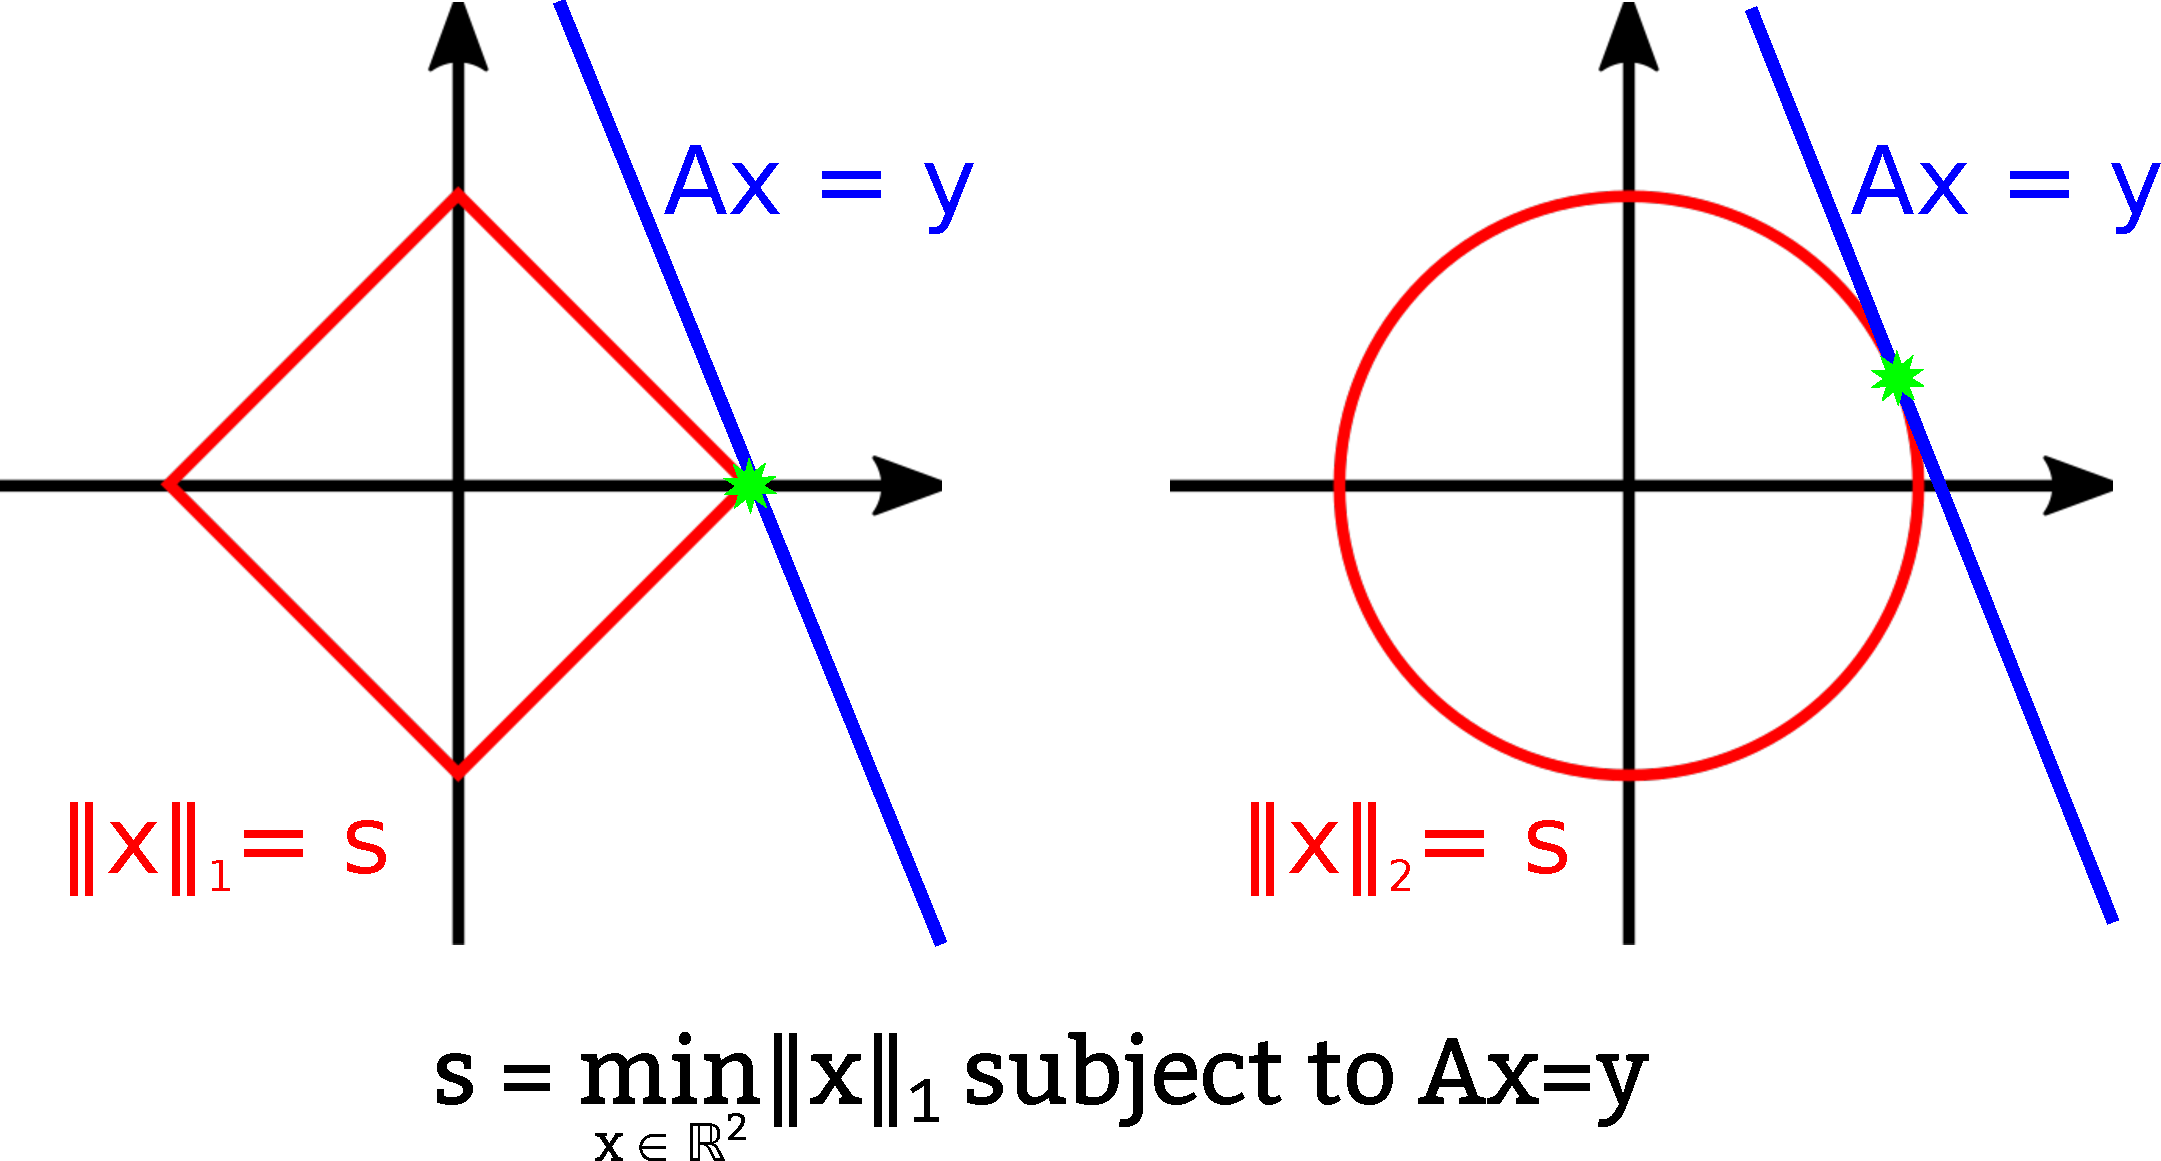
\includegraphics[width=0.7\linewidth]{images/sparse_solution.pdf}
        \caption{\textbf{Solution of $\ell_1$ and $\ell_2$ minimization problems.} Matrix $\mathbf{A} \in \mathbb{R}^{1 \times 2}$ is an underdetermined linear system, and the task is to find $\mathbf{x} \in \mathbb{R}^2$ with minimal $\ell_1$-norm such that it satisfies the equation $\mathbf{Ax} = \mathbf{y}$ for fixed $\mathbf{y} \in \mathbb{R}$. The number of solutions are infinite (all points along the blue line), and the unique solution of minimization problem is marked with a green star. Note that $\ell_1$ minimization gives sparse solution, while $\ell_2$ minimization is not sparsity seeking.}
        \label{fig:sparse_solution}
    \end{minipage}%
    \hspace{0.02\textwidth}
    \begin{minipage}{0.34\textwidth}
        \centering
        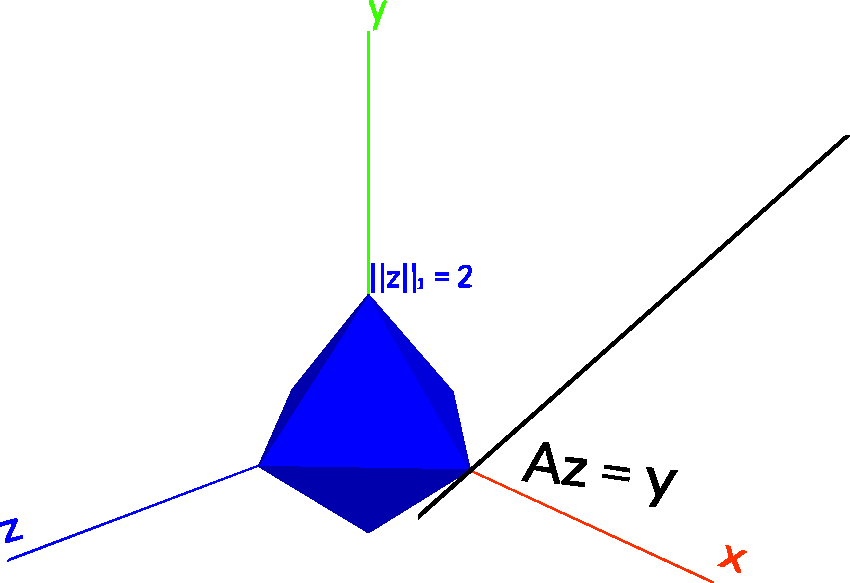
\includegraphics[width=\linewidth]{images/3D_l1_min.pdf}
        \caption{\textbf{$\ell_1$ minimization in 3D.} This figure demonstrates the sparsity seeking nature of $\ell_1$ minimization in a 3-dimensional space. The image is taken from the interactive demo available at \url{https://hakkelt.github.io/CS-demo/}}
        \label{fig:3D_l1_min}
    \end{minipage}
\end{figure}

\begin{definition}[NSP]
A matrix $\mathbf{A} \in \mathbb{C}^{m \times N}$ is said to satisfy the null space property (NSP) of order $s$, if for any set $S \subset [N]$ with $|S| = s$
\[\norm{\mathbf{v}_S}_1 < \norm{\mathbf{v}_{S^C}}_1 : \forall \mathbf{v} \in ker(\mathbf{A})  \setminus \{\mathbf{0}\}.\]
\end{definition}

\begin{notation}
For a vector $\mathbf{v} \in \mathbb{C}^N$ and a set $S \subset [N]$, we denote by $\mathbf{v}_S$ either the vector in $\mathbb{C}^{|S|}$ which is the restriction of $\mathbf{v}$ to the indices in $S$, or the vector in $\mathbb{C}^N$ which coincides with $\mathbf{v}$ on the indices in $S$ and is zero elsewhere. Similarly, $\mathbf{v}_{S^C}$ means the same with the complement of $S$.
\end{notation}

\begin{theorem}
Given a matrix $\mathbf{A} \in \mathbb{C}^{m \times N}$, every $s$-sparse vector $\mathbf{x} \in \Sigma_s^N \subset \mathbb{C}^N$ is the unique solution of (\ref{eq:P_1}) with $\mathbf{y} = \mathbf{Ax}$ if and only if $\mathbf{A}$ satisfies the NSP of order $s$.
\end{theorem}

\begin{remark}
This theorem shows that for every $\mathbf{y} = \mathbf{Ax}$ with $s$-sparse $\mathbf{x}$, the $\ell_1$-minimization (\ref{eq:P_1}) actually solves the $\ell_0$-minimization (\ref{eq:P_0}) when the NSP of order $s$ holds.
\end{remark}

Although NSP is a formidable construct that allows relatively easy and straightforward proofs, in realistic settings, signals are rarely sparse, but rather \textit{almost} $s$-sparse vectors, meaning that the most part of the energy of the signal is concentrated in $s$ coefficients with the the largest values. To involve these cases in the compressed sensing framework, an extension of NSP is used, called \textit{stable NSP}. Proving the stable NSP property, one can then approximate the almost $s$-sparse signal with the \textit{best $s$-term approximation} having a tight bound on the error term.

\begin{definition}[$\ell_p$-error of best $s$-term approximation]
For $p > 0$, the $\ell_p$-error of best $s$-term approximation to a vector $\mathbf{x} \in \mathbb{C}^N$ is defined by
\[\sigma_s(\mathbf{x})_p = \inf\left\{\norm{\mathbf{x} - \mathbf{z}}_p : \mathbf{z} \in \Sigma_s^N\right\}.\]
\end{definition}

\begin{remark}
The  infimum is always achieved by an $\mathbf{z} \in \Sigma_s^N$ whose non-zero entries equal the $s$ largest absolute entries of $\mathbf{x}$.
\end{remark}

\begin{definition}[stable NSP]
A matrix $\mathbf{A} \in \mathbb{C}^{m \times N}$ is said to satisfy the stable NSP with constant $0 < \rho < 1$ of order $s$, if for any set $S \subset [N]$ with $|S| = s$
\[\norm{\mathbf{v}_S}_1 \le \rho \norm{\mathbf{v}_{S^C}}_1 : \forall \mathbf{v} \in ker(\mathbf{A}).\]
\end{definition}

\begin{theorem}
The matrix $\mathbf{A} \in \mathbb{C}^{m \times N}$ satisfies the stable NSP with constant $0 < \rho < 1$ of order $s$ if and only if for any set $S \subset [N]$ with $|S| = s$
\begin{equation}\label{eq:stable_nsp}
    \norm{\mathbf{z} - \mathbf{x}}_1 \le \frac{1 + \rho}{1 - \rho} \left(\norm{\mathbf{z}}_1 - \norm{\mathbf{x}}_1 + 2\norm{\mathbf{x}_{S^C}}\right)
\end{equation}
holds for any set $S \subset [N]$ with $|S| = s$ and for all vectors $\mathbf{x,z} \in \mathbb{C}^N$ with $\mathbf{Az} = \mathbf{Ax}$.
\end{theorem}

\begin{remark}
The estimation (\ref{eq:stable_nsp}) can be upper-bounded by means of the $\ell_1$-error of best $s$-term approximation $\sigma_s(\mathbf{x})_1$ as
\[\norm{\mathbf{z} - \mathbf{x}}_1 \le \frac{1 + \rho}{1 - \rho} \left(\norm{\mathbf{z}}_1 - \norm{\mathbf{x}}_1 + 2\norm{\mathbf{x}_{S^C}}\right) \le 2 \cdot \frac{1 + \rho}{1 - \rho}\sigma_s(\mathbf{x})_1.\]
\end{remark}

The significance of this theorem is that it implies that having the stable NSP fulfilled, the unique $s$-sparse solution $\mathbf{z}$ of (\ref{eq:P_1}) with $\mathbf{y} = \mathbf{Ax}$ approximates the vector $\mathbf{x}$ with a bounded $\ell_1$-error. Therefore, by a good approximation of the sparsity $s$ of the signal and an upper bound $\epsilon$ of $\sigma_s(\mathbf{x})_1$ (both can be inferred by the statistics of the signal), one can construct or select a measurement matrix $\mathbf{A}$ such that the solution of \textit{any} algorithm solving (\ref{eq:P_1}) is an approximation of the input signal with the maximal error of
\[\frac{1 + \rho}{1 - \rho} \cdot 2\epsilon,\]
where $\rho$ depends only on the measurement matrix and $\epsilon$ is a small number because only little energy is stored in the entries contributing the the $\ell_p$-error of best $s$-term approximation.
Practically that means that by the careful design of the measurement, arbitrary precision recovery is possible (having Nyquist sampling as a special case for guaranteed perfect recovery), and that in case of approximately $s$-sparse signals, the number of measurements can be drastically reduced without significant amount of error introduced.

Finally, this construct can be further extended  to handle noisy measurement: proving the \textit{robust NSP} for the measurement matrix, the same guaranties apply to the $\ell_1$-error as in case of stable recovery, extended by an extra term characterizing the noise on the measurement. As a result, arbitrary precision is allowed for arbitrary optimization algorithm capable of solving (\ref{eq:P_1_noisy}) given a measurement matrix satisfying the \textit{robust NSP}.

\begin{definition}[robust NSP]
A matrix $\mathbf{A} \in \mathbb{C}^{m \times N}$ is said to satisfy the robust NSP with constants $0 < \rho < 1$ and $0 < \tau$ of order $s$, if for any set $S \subset [N]$ with $|S| = s$
\[\norm{\mathbf{v}_S}_1 \le \rho \norm{\mathbf{v}_{S^C}}_1 + \tau \norm{\mathbf{Av}}_2 : \forall \mathbf{v} \in \mathbb{C}^N.\]
\end{definition}

\begin{remark}
Note that $\mathbf{v}$ is not required to be in $ker(\mathbf{A})$.  In fact, if $\mathbf{v} \in ker(\mathbf{A})$, then $\mathbf{Av} = \mathbf{0}$, and we obtain the definition of stable NSP. Therefore, the robust NSP implies stable NSP.
\end{remark}

\begin{theorem}
The matrix $\mathbf{A} \in \mathbb{C}^{m \times N}$ satisfies the robust NSP with constants $0 < \rho < 1$ and $0 < \tau$ of order $s$ if and only if
\begin{equation}\label{eq:robust_nsp}
    \norm{\mathbf{z} - \mathbf{x}}_1 \le \frac{1 + \rho}{1 - \rho} \left(\norm{\mathbf{z}}_1 - \norm{\mathbf{x}}_1 + 2\norm{\mathbf{x}_{S^C}}\right) + \frac{2\tau}{1-\rho}\norm{\mathbf{A(z-x)}}_2
\end{equation}
holds for any set $S \subset [N]$ with $|S| = s$ and for all vectors $\mathbf{x,z} \in \mathbb{C}^N$ with $\mathbf{Az} = \mathbf{Ax}$.
\end{theorem}

\begin{remark}
Supposing that a matrix $\mathbf{A} \in \mathbb{C}^{m \times N}$ satisfies the robust NSP of order $s$, (\ref{eq:robust_nsp}) implies that for any $\mathbf{x} \in \mathbb{C}^N$, a solution $\mathbf{z}$ of (\ref{eq:P_1_noisy}) with $\norm{\mathbf{Ax - y}} \le \eta$ approximates $\mathbf{x}$ with $\ell_1$-error \footnote{Number $4$ in the numerator of the error term at (\ref{eq:error_bound}) is not a typo as one would expect, but a counterintuitive result of some basic arithmetics leading to this expression.}
\begin{equation}\label{eq:error_bound}
    \norm{\mathbf{z} - \mathbf{x}}_1 \le 2 \cdot \frac{1 + \rho}{1 - \rho}\sigma_s(\mathbf{x})_1 + \frac{4\tau}{1-\rho}\eta.
\end{equation}
\end{remark}

The main problem, nevertheless, with the NSP is that proving it is actually NP-hard in general. Hence, the \textit{restricted isometry property (RIP)} is more commonly used in theoretical works because it is easier to handle, and at the same time it implies stable NSP.

\begin{definition}[RIP]
A matrix $\mathbf{A} \in \mathbb{C}^{m \times N}$ is said to satisfy the $s$-restricted isometry property with the smallest number $0 < \delta_s < 1$, called restricted isometry constant (RIC), if
\[(1 - \delta_s)\norm{\mathbf{x}}_2^2 \le \norm{\mathbf{Ax}}_2^2 \le (1 + \delta_s)\norm{\mathbf{x}}_2^2\]
holds for add $\mathbf{x} \in \Sigma_s^N$.
\end{definition}

\begin{theorem}
If a matrix $\mathbf{A} \in \mathbb{C}^{m \times N}$ has restricted isometry constant 
\[\delta_{2s} < \frac{1}{\sqrt{2}},\] then it satisfies the robust NSP of order $s$ with constants
\[\rho = \frac{\delta_{2s}}{\sqrt{1 - \delta_{2s}^2}} \text{ and } \tau = \frac{2\sqrt{s}}{(1-\delta_{2s}\sqrt{1 + \delta_{2s}}}.\]
\end{theorem}

\subsection{The Connection Between CS and MRI}
Although it is not always trivial to apply the compressed sensing scheme to different measurement methods, MR imaging is in a lucky position with the Fourier transform in the core of its image acquisition process as random partial discrete Fourier transform (i.e., selecting $m$ rows randomly with uniform distribution from the $N$ rows, or in other words, observing only $m$ entries of the Fourier transform) is proved to satisfy the RIP~\cite{fornasier_theoretical_2010}. That discovery has enormous significance as is offers a way to speed up the inherently slow MRI measurements by measuring only a few randomly selected points from the k-space, and then solve the $\ell_1$-minimization problem via an arbitrarily selected optimization algorithm.

\begin{figure}[htbp]
    \centering
    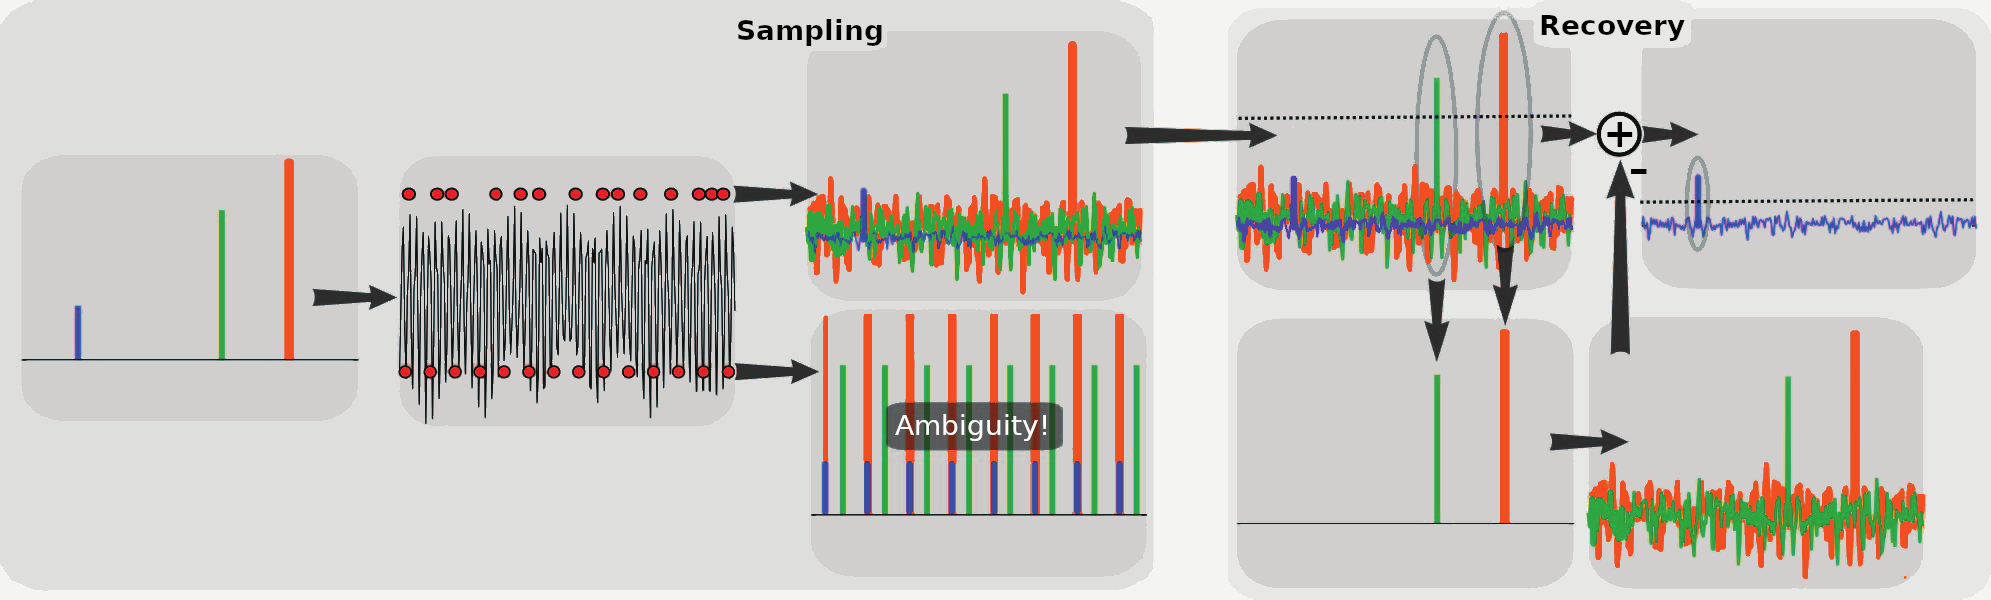
\includegraphics[width=0.9\linewidth]{images/random_sampling.png}
    \caption{\textbf{A heuristic reconstructing signal from random undersampling.} In the left block, the result of Fourier analysis is shown for both equidistant and random sampling, demonstrating the underdetermined nature of equidistant undersampling (bottom) and the noise-like effect of random sampling (top). In the right block, a simple method is applied that selects the peaks above a certain threshold as candidates, calculates the inference of these peaks, and substracts the calculated inference from the spectrum allowing detection of further peaks after lowering the threshold. Source: Adapted from~\cite{lustig_compressed_2008}.}
    \label{fig:random_sampling_1D}
\end{figure}

\begin{figure}[htbp]
    \centering
    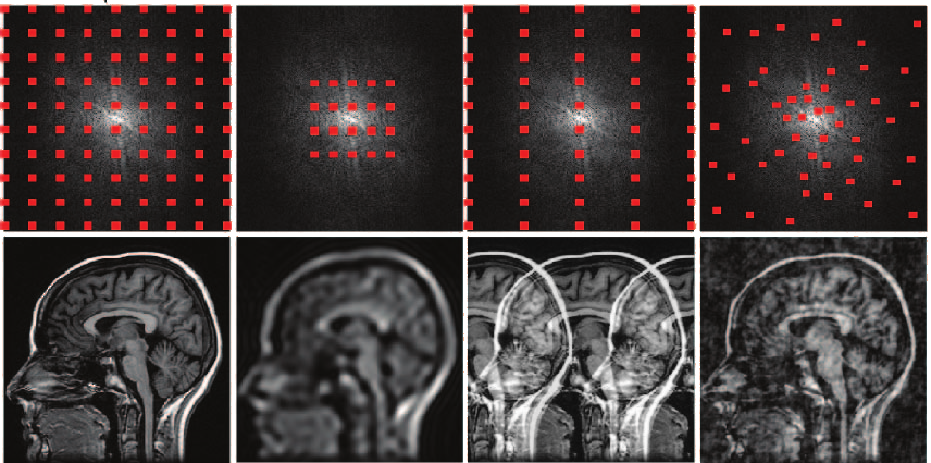
\includegraphics[width=0.8\linewidth]{images/random_sampling2.png}
    \caption{\textbf{Connection between the sampling pattern and the introduced inference.} Using inverse DFT replacing the missing values with zeros leads to different type of undersampling artifacts. Sampling only the center reduces the resolution, undersampled equispaced scheme adds shifted copies of the signal to the recovered image, and random sampling spreads the inference uniformly. Source: Adapted from~\cite{lustig_compressed_2008}.}
    \label{fig:random_sampling_images}
\end{figure}

One can think of this recovery scheme as a denoising or inference cancelling process where the noise/inference to be removed is the sum of undersampling artifacts predicted by Nyquist-Shannon theorem. If we use an equispaced sampling pattern, then the resulted noise is basically shifted copies of the signal and hence recovery of the original signal is impossible as each replica is an equally likely candidate. Figure~\ref{fig:random_sampling_1D} illustrates this problem and demonstrates the advantage of random sampling. In contrast, random sampling "spreads" the noise uniformly over the image, so the inference acts mostly like white noise (see fig.~\ref{fig:random_sampling_images}). This approach is particularly appealing as countless denoising algorithms exists, and as many of them are based on minimization of the $\ell_1$-norm of the transform of signal, these methods provide a convenient way to solve (\ref{eq:P_1}) problem. The transform used is always depends on the type of image in interest: MR angiograms (imaging technique visualizing blood vessels) are sparse even in the image domain, but edge detection algorithms like finite differences transform (that corresponds to the well-known total variation (TV) penalty) can further enhance sparsity (fig.~\ref{fig:MRA}); brain images have a sparse representation in various wavelet transformations~\ref{fig:brain_wavelet}, and dynamic MR images tend to be sparse after temporal Fourier transform is applied.

\begin{figure}[htbp]
    \centering
    \begin{minipage}[t]{0.65\linewidth}
        \centering
        \begin{tabular}{c}
            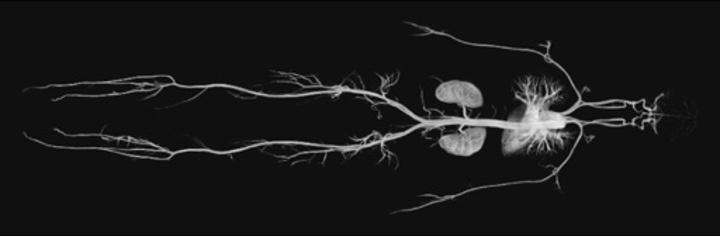
\includegraphics[width=0.95\linewidth]{images/MRI-Angiography.jpg}
            \\
            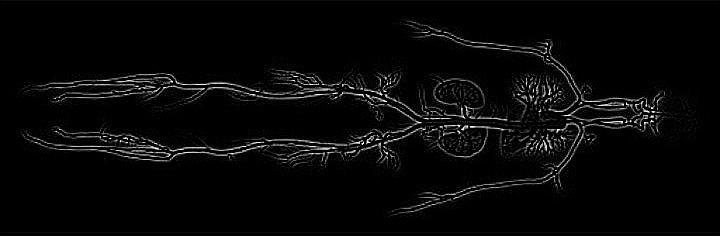
\includegraphics[width=0.95\linewidth]{images/MRI-Angiography_edges.jpg}
        \end{tabular}
        \caption{\textbf{MR angiograms} (MR images tuned to show blood vessels) are intrinsically sparse even in image domain (top image), but sparseness can be further improved by edge detection algorithms (botton image) because only the morphology of the blood vessels are diagnostically relevant. Source: Adapted from~\cite{noauthor_mri_nodate}.}
        \label{fig:MRA}
    \end{minipage}
    \hspace{0.02\linewidth}
    \begin{minipage}[t]{0.31\linewidth}
        \centering
        \begin{tabular}{c}
            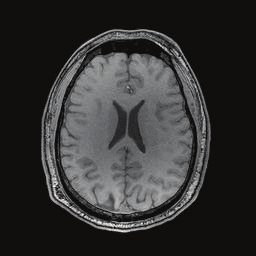
\includegraphics[width=0.65\linewidth]{images/brain_MRI.png}
            \\ 
            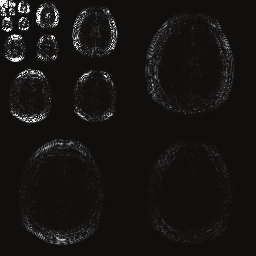
\includegraphics[width=0.65\linewidth]{images/brain_MRI_wavelet.png}
        \end{tabular}
        \caption{\textbf{MRI images of the brain} are not sparse in image domain, but they are in multiple wavelet transform domains. Source:~\cite{zhao_compressed_2014}.}
        \label{fig:brain_wavelet}
    \end{minipage}
\end{figure}

A truly random sampling in the k-space, however, is generally impractical due to hardware and physiological constraints. For example, the sampling must follow smooth lines and curves and be robust to real-life situations such as motion artifacts. Also, a uniform random distribution of samples in the spatial-frequency domain does not take into account the energy distribution of MR images in k-space. Therefore it makes more sense to opt for a nonuniform variable density sampling matching energy distribution in k-space. Precisely, we should consider having more samples from the central part of the frequency domain and less high frequency components. Consequently, carefully designed pseudo-random sampling trajectories are utilized in practice. To quantify  evaluate the "randomness" of the trajectories, authors of~\cite{lustig_compressed_2008} and~\cite{lustig_sparse_2007} suggested using point spread function (PSF) to measure the desirable incoherence of the aliasing interference, defined as
\[PSF = (\mathbf{e}_j^* \mathcal{F}_u^* \mathcal{F}_u \mathbf{e}_i)_{i,j}\]
where $\mathcal{F}_u$ is the undersampling Fourier transform operator, $\mathbf{e}_i$ and $\mathbf{e}_j$ are of the natural basis having $0$ in each coordinate except the $i$-th and $j$-th position, resprectively, where $1$ is located. Thus, $PSF_{i,j}$ measures the contribution of a unit-intensity pixel at the $i$-th position of the image to the $j$-th position in the k-space. In case of fully sampled measurement, the $PSF$ is an identity matrix, and undersampling induces non-zero off-diagonal terms. Figuratively speaking, $PSF$ measures the leakage of energy from a Kronecker delta input. Figure~\ref{fig:trajectory_coherence} shows $PSF$ for a central pixel for a couple sampling trajectories. This quantitiy then can serve as a simple measure for the incoherence by calculating the sidelobe-to-peak ratio:
\[SPR = \max_{i \ne j} \left|\frac{PSF_{i,j}}{PSF_{i,i}}\right|.\]
As a result, the design of an incoherent sampling trajetory aims to minimize $SPR$.

\begin{figure}
    \centering
    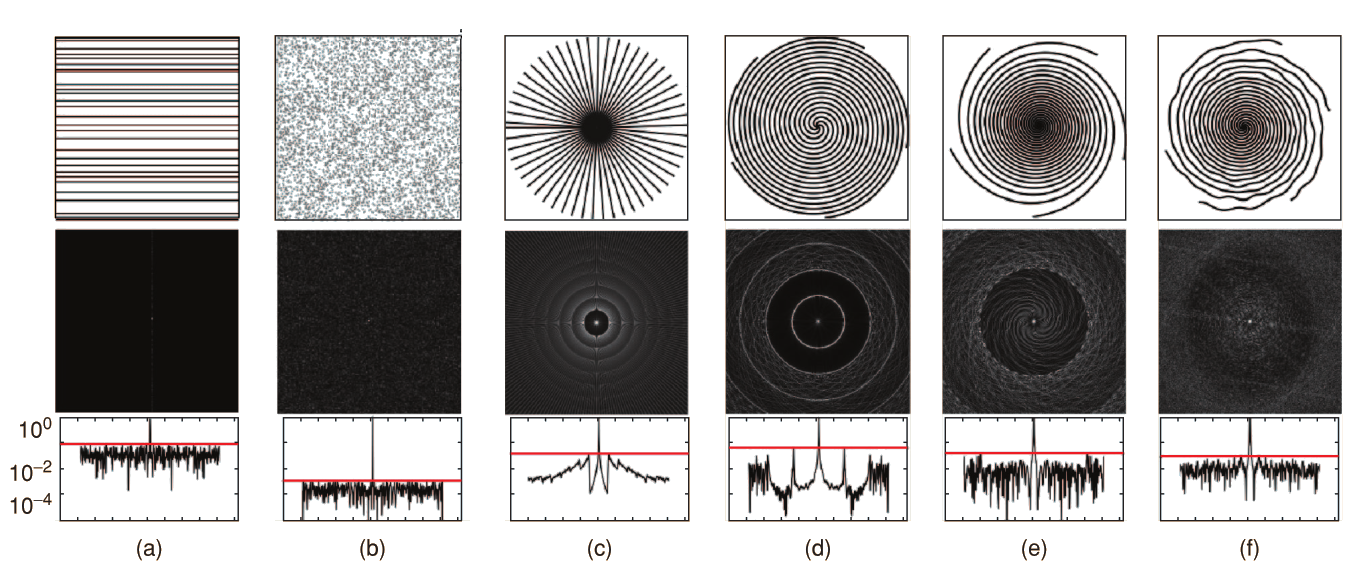
\includegraphics[width=0.98\linewidth]{images/PSF_trajectories.png}
    \caption{\textbf{$\mathbf{PSF}$ of the central pixel for various sampling trajectories:} (a) randomly chosen horizontal lines, (b) uniformly selected random points, (c) radial, (d) uniform spirals, (e) variable density spirals, and (f) variable density perturbed spirals. The red line marks the overall coherence level.\\
    Source: Adapted from~\cite{lustig_compressed_2008}.}
    \label{fig:trajectory_coherence}
\end{figure}

\section{Numerical Methods}

While the recovery is proved to be \textit{possible} via polynomial time algorithms minimizing the $\ell_1$-relaxation of ($\ref{eq:P_0}$), finding the best algorithm for a given use-case is a quite challenging problem as the algorithm must satisfy many constraints like fast convergence speed and guarantee for a (global) convergence, inexpensive computation and limited memory requirement, numerical robustness and lack of problem-dependent parameters. The number of choices are numberless; nevertheless, none of them appears to outperform all other in every aspects because improving convergence speed while keeping global convergence is difficult, increased computational speed usually comes at the cost of a more memory hungry implementation, and it is hard to optimize algorithms without tuning its parameters specifically to the problem to be solved.

The computation cost and the memory requirement, in particular, tend to be most restrictive constraint. Namely, the direct calculation of Hessian is often computationally prohibitive on one hand, on the other hand, the storage of the calculated Hessian can be problematic even for medium sized images. To see that, let us consider a $256 \times 256$ grayscale image. Storing all the $65536$ pixels of the image as a half-precision floating point number requires $256 \times 256 \times \SI{2}{\byte} = \SI{128}{\kibi\byte}$. While the gradient of the image is of the same size, the Hessian has a quadratic memory requirement, $(256 \times 256)^2 \times \SI{2}{\byte} = \SI{8}{\gibi\byte}$ in our example. Although this requirement can be satisfied even on a stronger personal computer, a high-resolution dynamic MR image, for instance, usually results in magnitudes larger allocations, like \SI{256}{\gibi\byte} for a 3D image of size $512\times512\times512$ with 512 time frames and an enormously large \SI{33554432}{\tebi\byte} allocation for its Hessian. 

Therefore, second order optimization algorithms (i.e., algorithms using second derivative) are not feasible in image reconstruction problems in general, even though these algorithms usually outperform first order methods in convergence speed. On the other end of the scale, zeroth order methods (that is, algorithms not using any gradient information), while being feasible and sometimes used for image reconstruction, are considered to be impractical due to their slow convergence. Therefore, first order methods appear to be the default option in nearly all image processing settings, and accordingly, we will discuss them exclusively in the following. Of course, even this restricted scope is far too large to cover, hence we restrict ourselves only to a few concepts that will serve as building blocks of more complex algorithms reviewed in the next chapters.

\subsection{General Gradient Descent}
Since Cauchy first proposed an iterative gradient direction method to solve astronomic calculations in 1847~\cite{cauchy_methode_1847}, the family of gradient descent algorithms became one of the largest and most popular group of solvers due to their simplicity and relatively inexpensive computation. The core of all gradient methods is the so called gradient step defined as
\[\mathbf{x}_{k+1} = \mathbf{x}_k + \alpha_k \nabla f(\mathbf{x_k}),\]
where $f$ is commonly called a loss or cost function, and $\alpha$ is generally referred to as step size and it is a negative number if we consider the minimization problem and positive if we are looking for the maximum.

The greatest advantage of gradient descent is that it is universally applicable to all problems where $f$ is differentiable, but it is capable to find only a local optimum, and, in its original form, it is rarely optimal (albeit sometimes the only feasible option). Additionally, finding the optimal step size and a proper starting point is quite challenging, and convergence is not always guaranteed. If the step size is too small then the convergence speed becomes impractically slow; on the other hand, too large step size can make the algorithm fail to converge. The improper choice of the initial point can also drastically delay convergence, and also might cause converge to a unfavorable local optimum instead of the global optimum (or, at least, a better optimum nearby).

\subsubsection{Selection of Step Size}
While a good starting point is always depends on the function to be minimized (from this point, we consider only the minimization problem without loss of generality), there are various schemes for determining the step size in each step. Notably, the line search methods are commonly used to solve this problem because of its universally applicability. As the name suggests, these methods perform a search for local minimum along a descent direction (which, in case of gradient methods, is given by the gradient) and return exactly the step size needed to step into this minimum. The search can be exact (like the later described conjugate gradient' implicit line search) or inexact where only an approximation of the local minimum is calculated (like backtracking line search~\cite{armijo_minimization_1966} (see also fig.~\ref{fig:backtracking}) or using Wolfe conditions~\cite{wolfe_convergence_1969}).

However, the line search methods become impractical when evaluation of the cost function is computationally expensive. In these cases only fixed (but not necessarily constant) step is applicable. Restricting the cost function to the set of convex and smooth (differentiable with $L$-Lipschitz-gradient) functions, the analysis of global convergence of first order methods with respect to step size selection becomes possible, still covering a very large part of practical problems. In the following, $f$ is always assumed to satisfy these conditions.

The simplest step size selection scheme is the constant step size, and if we choose the step size to be $\frac{1}{L}$ where $L$ is the Lipschitz constant of $\nabla f$, then monotonic descent is ensured and convergence to the global minimizer is guaranteed  as $f$ is assumed to be convex. The convergence rate of cost function is linear ($\mathcal{O}(1/k)$) as 
\[f(\mathbf{x}_k) - f(\mathbf{x}_*) \le \frac{L\norm{\mathbf{x}_0 - \mathbf{x}_*}}{4k + 2}\]
is proved to be a tight inaccuracy bound for the generated sequence~\cite{drori_performance_2014}. This rate, however, is undesirably slow, and therefore the optimal step size is a highly researched topic. Although it was only recently proved that the convergence rate of all first order method with constant step size is still linear at best~\cite{taylor_smooth_2017}, there is already a long history of accelerated gradient methods like conjugate gradient, heavy ball iterations, and fast gradient method.

\subsection{Conjugate Gradient Method}

To overcome the slow convergence rate of the classic gradient descent (GD) method, one can use a modified version of it, the conjugate gradient method (CG) developed by Hestenes and Stiefel~\cite{hestenes_methods_1952}, if the problem is defined by a symmetric (or self-adjoint in complex case) and positive-definite matrix. In that case, the direction of movement must be conjugate to the previous directions. Two non-zero vectors $\mathbf{u}$ and $\mathbf{v}$ are conjugate with respect to some $\mathbf{A}$ matrix, if \[\mathbf{u}^T\mathbf{Av} = \mathbf{0}.\]
Let us consider the following linear system as the subject of optimization:
\[\mathbf{Ax} = \mathbf{b},\]
where $\mathbf{A} $is symmetric, positive-definite and real matrix, and $\mathbf{b}$ is also known.

\subsubsection{As a direct method} Since $\mathbf{A}$ is symmetric and positive-definite, it defines an inner product:
\[\langle \mathbf{u}, \mathbf{v} \rangle_\mathbf{A} := \mathbf{u}^T\mathbf{Av}.\]
Using that inner product, it is possible to find $n$ pairwise conjugate vectors: $\mathcal{P} = \{\mathbf{p}_1,...\mathbf{p}_n\}$. Then $\mathcal{P}$ forms a basis in $\mathbb{R}^n$, so the solution ($\mathbf{x_*}$) of optimization problem can be represented in terms of that basis:
\begin{equation} \label{eq:direct_method}
    \mathbf{x_*} = \sum_{i=1}^{n} \alpha_i \mathbf{p}_i.
\end{equation}
Left multiplying both sides with $\mathbf{p}_k^T \mathbf{A}$ we get:
\[\mathbf{p}_k^T\mathbf{Ax_*} = \sum_{i=1}^{n} \alpha_i \mathbf{p}_k^T \mathbf{A} \mathbf{p}_i = \sum_{i=1}^{n} \alpha_i \langle \mathbf{p}_k, \mathbf{p}_i \rangle_\mathbf{A}.\]
As we know that $\mathbf{Ax_*} = \mathbf{b}$ and that $\langle \mathbf{p}_k, \mathbf{p}_i \rangle_\mathbf{A} = 0 : \forall i \ne k $  because $\mathbf{p}_i$ vectors are mutually conjugate (i.e. orthogonal with respect to the inner product defined by matrix $\mathbf{A}$):
\[\mathbf{p}_k^T\mathbf{b} = \alpha_k \langle \mathbf{p}_k^T, \mathbf{p}_k \rangle_\mathbf{A}.\]
That way we can calculate all $\alpha_i$ coefficients,:
\[\alpha_i = \frac{\mathbf{p}_i^T\mathbf{b}}{\langle \mathbf{p}_i, \mathbf{i}_k \rangle_\mathbf{A}},\]
and using these coefficients $\mathbf{x_*}$ can be calculated directly by equation \ref{eq:direct_method}.

\subsubsection{As an iterative method} One weakness of direct method that for high dimensional vectors, we have to calculate high number of coefficients. On the other hand, it is not necessary to calculate all of them as a good approximation of $\mathbf{x_* }$ can be obtained using only a few well chosen $\mathbf{p_i}$ vectors. To achieve that we need to define a cost function:
$$f(\mathbf{x}) = \frac{1}{2}\mathbf{x}^T \mathbf{Ax} - \mathbf{x}^T \mathbf{b}.$$
The existence of a unique minimizer is evident as its second derivative is given by a symmetric positive-definite matrix:
\[\nabla^2 f(\mathbf{x}) = \mathbf{A}.\]
Also, we can calculate the first derivative easily:
\[\nabla f(\mathbf{x}) = \mathbf{Ax} - \mathbf{b}.\]
After choosing an arbitrary starting point $\mathbf{x}_0$, we can start the iteration by calculating the so called \textit{residual}, which is apparently equal to the negative gradient:
\[\mathbf{r}_{k+1} = \mathbf{b} - \mathbf{Ax}.\]
Then we have to make sure to get a direction that is conjugate to all previous directions by applying an operation similar to the Gram-Schmidt orthonormalising:
\[\mathbf{p}_k = \mathbf{r}_k - \sum_{i<k} \frac{\langle \mathbf{p}_i, \mathbf{r}_k \rangle_\mathbf{A}}{\langle \mathbf{p}_i, \mathbf{p}_i \rangle_\mathbf{A}} \mathbf{p}_i.\]
Following this direction, the next optimal location is given by
\[\mathbf{x}_{k+1} = \mathbf{x}_k + \alpha_k \mathbf{p}_k,\]
where $\alpha_k$ can be derived by substituting the previous formula for $\mathbf{x}_{k+1}$ to the the cost function and minimizing it with respect to $\alpha_k$ :
\[\nabla f(\mathbf{x}_{k+1}) = \nabla f(\mathbf{x}_k + \alpha_k \mathbf{p}_k)  \overset{!}{=} 0 \Rightarrow ... \Rightarrow \alpha_k = \frac{\mathbf{p}_k^T \mathbf{r}_k}{\langle \mathbf{p}_k, \mathbf{p}_k \rangle_\mathbf{A}}\]
An example that gives an intuition why CG needs less steps than GD is shown by fig.~\ref{fig:grad_desc_problem} where the inappropriate step size and a "curved valley" produce zigzagging motion, and slow convergence as a result, which is slowed even further when the flat area in the bottom of that valley is reached. In contrast, CG avoids zigzagging because of the constraint of conjugate directions as it is depicted on fig.~\ref{fig:CG_vs_GD}.

\begin{figure}
    \centering
    \begin{minipage}[t]{0.40\linewidth}
        \centering
        \includegraphics[width=.8\linewidth]{images/backtracking.png}
        \caption{\textbf{Example for backtracking algorithm.} This 2D section of a high dimensional function is selected by the gradient direction, and we are looking for the local minimum along that slice. In the first step, a relatively large step size is chosen, which gets gradually decreased until local minimum is reached.}
        \label{fig:backtracking}
    \end{minipage}
    \hspace{0.01\linewidth}
    \begin{minipage}[t]{0.255\linewidth}
        \centering
        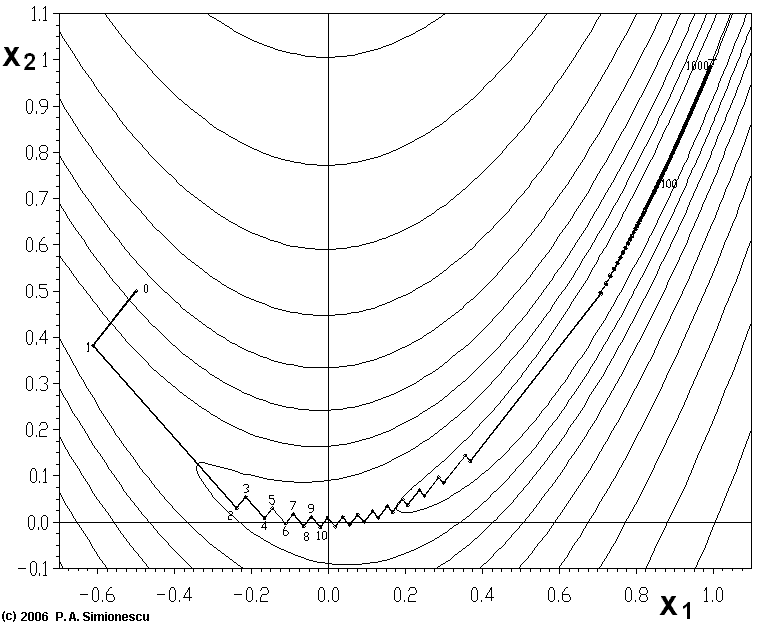
\includegraphics[width=\linewidth]{images/Banana-SteepDesc.png}
        \caption{Example of the effect of inappropriate step size, "curved valley" and flat area: slow convergence of gradient descent method. Source:~\cite{simionescu_illustration_2006}.}
        \label{fig:grad_desc_problem}
    \end{minipage}
    \hspace{0.01\linewidth}
    \begin{minipage}[t]{0.29\linewidth}
        \centering
        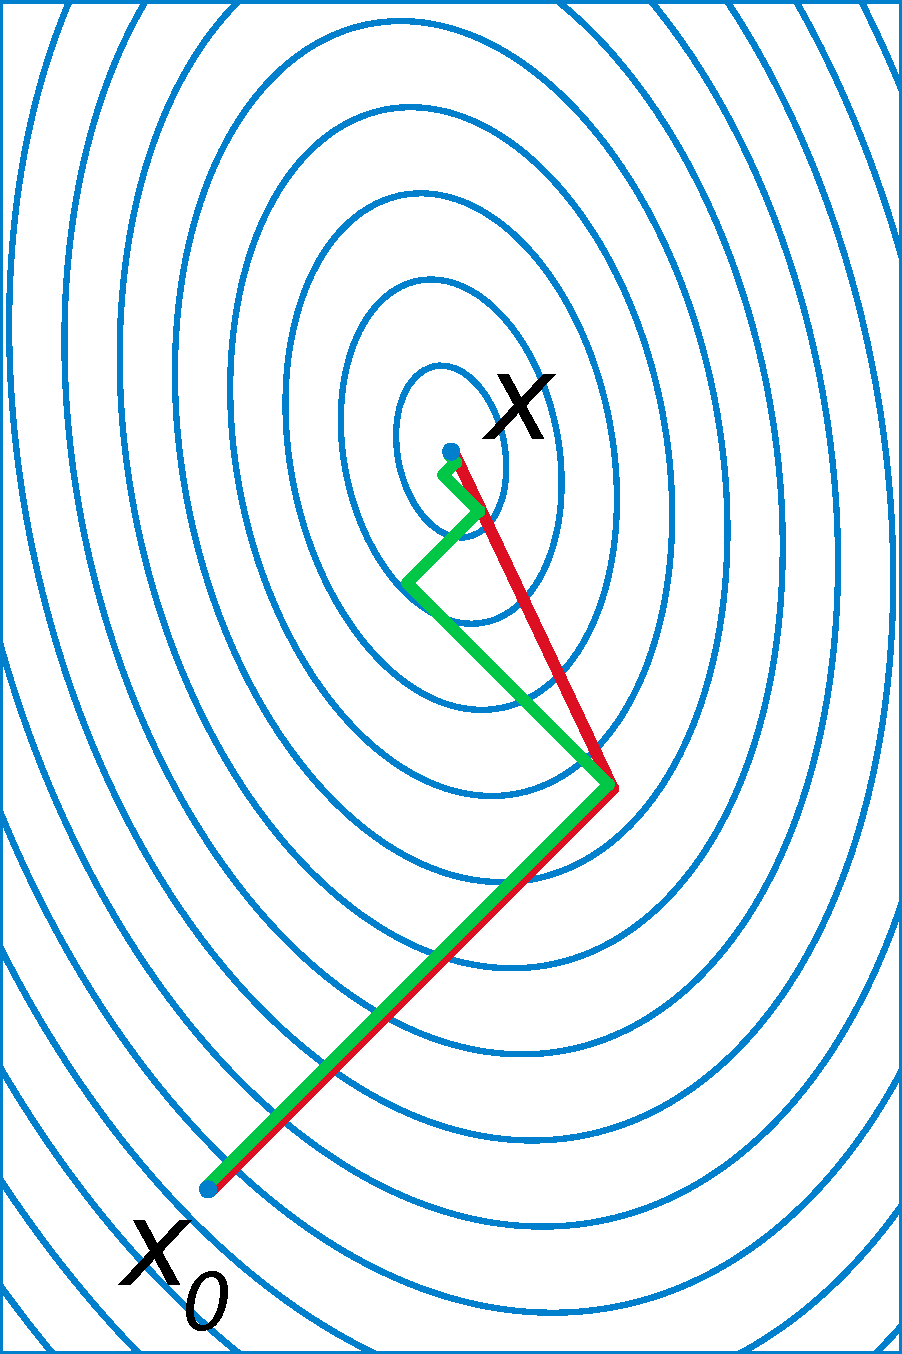
\includegraphics[width=0.45\linewidth]{images/Conjugate_gradient_illustration.pdf}
        \caption{Visualization of the advantage of the CG method compared to GD: CG requires significantly fewer steps. The green line shows the path of the GD method, red shows the path of the CG method. Source:~\cite{alexandrov_illustration_2007}.}
        \label{fig:CG_vs_GD}
    \end{minipage}
\end{figure}

The basic algorithm, but still the most popular version, can be simply summarized as follows:

\begin{algorithm}[H]
    \SetKwInOut{Inputs}{input}
    \SetKwInOut{Output}{output}
    \Inputs{vector $\mathbf{b}$ ,\\ symmetric, positive-definite matrix $\mathbf{A}$, \\ $\epsilon \in \mathbb{R}_+$ error tolerance parameter, and \\ approximate initial solution $\mathbf{x}_0$ (optional, set to $\mathbf{0}$ by default)}
    \Output{vector $\mathbf{x}$ such that $\mathbf{Ax} = \mathbf{b}$}
    \BlankLine
    Initialize $\mathbf{r}_0 = \mathbf{b} - \mathbf{Ax}_0$, $\mathbf{p}_0 = \mathbf{r}_0$, $k = 0$\\
    \While{$\norm{\mathbf{r}_k} > \epsilon$}{
        $\alpha_k = \frac{\mathbf{r}_k^* \mathbf{r}_k}{\mathbf{p}_k^* \mathbf{Ap}_k}$\\
        $\mathbf{x}_{k+1} = \mathbf{x}_k + \alpha_k \mathbf{p}_k$\\
        $\mathbf{r}_{k+1} = \mathbf{r}_k - \alpha\mathbf{Ap}_k$\\
        $\beta_k = \frac{\mathbf{r}_{k+1}^* \mathbf{r}_{k+1}}{\mathbf{r}_k^* \mathbf{r}_k}$\\
        $\mathbf{p}_{k+1} = \mathbf{r}_{k+1} + \beta_k\mathbf{p}_k$\\
        $k = k + 1$
    }
    \Return $\mathbf{x}_k$
    \caption{Conjugate Gradient (CG) method}
\end{algorithm}

It worth noting that while it is hard to find a better method for simple problems than CG, in more complex cases preconditioning is necessary to ensure fast convergence. Furthermore, there exist multiple extensions of the base CG algorithm, like the biconjugate gradient (BiCG) method and its stabilized version (BiCGSTAB)~\cite{van_der_vorst_bicgstab_1992} that removes the constraint of self-adjointness, and the non-linear versions (just to name a few: \cite{fletcher_function_1964, polak_note_1969, dai_nonlinear_1999}) that pushes even further the boundary of set of problems solvable by CG.

\subsection[Accelerated Gradient Methods]{Accelerated Gradient Methods\footnote{This section follows the presentation~\cite{kim_optimal_2017} given by Jeffrey Fessler in December, 2017.}}

Even though the conjugate gradient methods provides an effective way to accelerate the convergence, the momentum-based methods that mostly outperform them in cases of complex, non-quadratic cost functions has also a long history. First, the so called heavy ball momentum was proposed by Polyak in 1967 to accelerate convergence~\cite{polyak_methods_1964}. The resulting heavy ball iteration takes the following form:
\[\mathbf{x}_{k+1} = \mathbf{x}_k - \frac{\alpha}{L}\nabla f(\mathbf{x}_k) + \beta (\mathbf{x}_k - \mathbf{x}_{k-1})\]
where $\alpha$ and $\beta$ are simple constants, and the term $\beta (\mathbf{x}_k - \mathbf{x}_{k-1})$ is referred to as the \textit{momentum}. The names \textit{heavy ball} and \textit{momentum} comes from the physical analogy; namely, the path defined by the minimizer sequence $\{\mathbf{x}_k\}$ resembles the route of a ball rolling down from a hill. The optimal choice of $\alpha$ and $\beta$ is unfortunately not trivial. In fact, universally optimal options not exists, but there are many variants of heavy ball method with different choice of $\alpha$ and $\beta$, being optimal always only in specific use cases. Following that, Nesterov published the algorithm in 1983 that later became known as fast gradient method (FGM)~\cite{nesterov_method_1983}. In contrast to the original gradient descent scheme, it maintains two converging sequences $\{\mathbf{x}_k\}$ and $\{\mathbf{z}_k\}$, of which $\{\mathbf{x}_k\}$ is the sequence that converges to the solution. The algorithm consists of three simple steps as shown below.

\begin{algorithm}[H]
    \SetKwInOut{Input}{input}
    \SetKwInOut{Output}{output}
    \Input{convex and smooth function $f$, \\ $\epsilon \in \mathbb{R}_+$ error tolerance parameter, and approximate initial solution $\mathbf{x}_0$ (optional, set to $\mathbf{0}$ by default)}
    \Output{vector $\mathbf{x} = \argmin f(\mathbf{x})$}
    \BlankLine
    Initialize $t_0 = 1, k = 0, \mathbf{z}_0 = \mathbf{x}_0$\\
    \Repeat{$\norm{\mathbf{x}_k - \mathbf{x}_{k-1}} < \epsilon$}{
        $\mathbf{z}_{k+1} = \mathbf{x}_k - \frac{1}{L}\nabla f(\mathbf{x}_k)$\\
        $t_{k+1} = \frac{1}{2}\left(1 + \sqrt{1 + 4t_k^2}\right)$\\
        $\mathbf{x}_{k+1} = \mathbf{z}_{k+1} + \frac{t_k - 1}{t_{k+1}}(\mathbf{z}_{k+1} - \mathbf{z}_k)$\\
        $k = k+ 1$
    }
    \Return{$\mathbf{x}$}
    \caption{Fast Gradient Method (FGM)}
\end{algorithm}

Despite the seemingly different formulations, both methods use some kind of momentum rule. The main difference is that heavy ball simply performs a weighted addition of the momentum from the previous iterations and the gradient of the current position, Nesterov's method combines these term in a couterintuitive, yet optimal manner as depicted on fig.~\ref{fig:momentum}. While FGM is preferred in convex optimization problems since it is slightly faster than heavy ball method, the latter is more commonly used in the machine learning community due to its robustness in non-convex settings.

\begin{figure}[t]
    \centering
    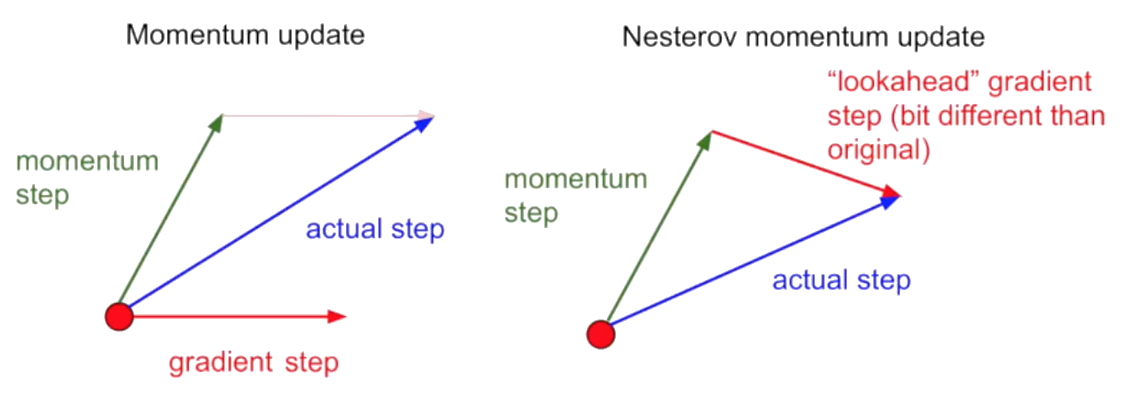
\includegraphics[width=0.8\linewidth]{images/momentum.png}
    \caption{\textbf{Difference between heavy ball momentum and Nesterov's momentum:} While the heavy ball simply performs a weighted addition of the momentum from the previous iterations and the gradient of the current position, Nesterov's method combines these term in a couterintuitive, yet optimal manner. Source: Image is adapted from~\cite{chandradevan_evolution_2017} and the idea of intuitive description of Nesterov's momentum rule as "lookahead" gradient step originates from~\cite{sutskever_importance_2013}.}
    \label{fig:momentum}
\end{figure}

Up to recent time, FGM was considered to be the fastest possible first order method for convex optimization because of its quadratic convergence proved by Nesterov. He also proved that the \textit{order} of convergence (i.e., quadratic convergence) of his algorithm is optimal indeed for first order methods. Nevertheless, the \textit{rate} of convergence of FGM is slightly sub-optimal as it was suggested by the convergence analysis performed by Drori and Teboulle in 2014~\cite{drori_performance_2014}. In their research, they considered a "meta optimization" problem, notably the minimization of worst-case convergence rate over all first order methods and all possible cost functions. As this problem is too difficult to be solved, they relaxed the problem to get a similar "meta-minimization" which can be solved by a semi-definite program. They found numerically that the relaxed bound of worst-case convergence rate for FGM is slightly below
\[\frac{2L\norm{\mathbf{x}_0 - \mathbf{x}_*}_2^2}{(N+1)^2},\]
where $N$ is the number of steps performed. Instead, they proposed a sequence of fixed step sizes calculated numerically that has approx. two times lower worst-case upper bound on convergence. Their approach, however, has a few drawbacks, such as the number of steps must be chosen in advance to ensure the improved convergence bound, and the numerical method producing these optimal step sizes is expensive both computationally and memory-wise. The next step that made this algorithm applicable in practical problems was done by Kim and Fessler in 2016, when they presented the analytical solution for the optimized step size coefficients~\cite{kim_optimized_2016} in the following form:

\begin{algorithm}[H]
    \SetKwInOut{Input}{input}
    \SetKwInOut{Output}{output}
    \Input{convex and smooth function $f$, \\ $\epsilon \in \mathbb{R}_+$ error tolerance parameter, and \\ approximate initial solution $\mathbf{x}_0$ (optional, set to $\mathbf{0}$ by default)}
    \Output{vector $\mathbf{x} = \argmin f(\mathbf{x})$}
    \BlankLine
    Initialize $\theta_0 = 1, k = 0, \mathbf{z}_0 = \mathbf{x}_0$\\
    \While{$\norm{\mathbf{x}_k - \mathbf{x}_{k-1}} > \epsilon$}{
        $\mathbf{z}_{k+1} = \mathbf{x}_k - \frac{1}{L}\nabla f(\mathbf{x}_k)$\\
        $\theta_k = \begin{cases}
            \frac{1}{2}\left(1 + \sqrt{1 + 4\theta_{k-1}^2}\right) : k = 1, 2, \ldots N - 1\\
            \frac{1}{2}\left(1 + \sqrt{1 + 8\theta_{k-1}^2}\right) : k = N
        \end{cases}$\\
        $\mathbf{x}_{k+1} = \mathbf{x}_k - \frac{1 + t_k/t_{k+1}}{L}\nabla f(\mathbf{x}_k) + \frac{t_k - 1}{t_{k+1}}(\mathbf{z}_{k+1} - \mathbf{z}_k)$\\
        $k = k + 1$
    }
    \Return{$\mathbf{x}$}
    \caption{Optimized Gradient Method 1 (OGM1)}
\end{algorithm}

This form reflects the simple modification of the existing Nesterov method that leads to the improved speed, namely the introduction of a new momentum term. The only problem is that the step size sequence still depends on the number of steps performed. Therefore, the same authors published a refined version of the algorithm~\cite{kim_convergence_2017} a year later that removes this limitation and also simplifies the implementation:

\begin{algorithm}[H]
    \SetKwInOut{Input}{input}
    \SetKwInOut{Output}{output}
    \Input{convex and smooth function $f$, \\ $\epsilon \in \mathbb{R}_+$ error tolerance parameter, and \\ approximate initial solution $\mathbf{x}_0$ (optional, set to $\mathbf{0}$ by default)}
    \Output{vector $\mathbf{x} = \argmin f(\mathbf{x})$}
    \BlankLine
    Initialize $t_0 = 1, k = 0, \mathbf{z}_0 = \mathbf{x}_0$\\
    \While{$\norm{\mathbf{x}_k - \mathbf{x}_{k-1}} < \epsilon$}{
        $\mathbf{z}_{k+1} = \mathbf{x}_k - \frac{1}{L}\nabla f(\mathbf{x}_k)$\\
        $t_{k+1} = \frac{1}{2}\left(1 + \sqrt{1 + 4t_k^2}\right)$\\
        $\mathbf{x}_{k+1} = \mathbf{x}_k - \frac{1 + t_k/t_{k+1}}{L}\nabla f(\mathbf{x}_k) + \frac{t_k - 1}{t_{k+1}}(\mathbf{z}_{k+1} - \mathbf{z}_k)$\\
        $k = k + 1$
    }
    \Return{$\mathbf{x}$}
    \caption{Optimized Gradient Method 2 (OGM2)}
\end{algorithm}

Of course, this formulation also enjoys the twice better worst-case convergence rate meaning that the new convergence bound on the helper sequence $\{\mathbf{z}_k\}$ for every iteration is
\[f(\mathbf{z}_k) - f(\mathbf{z}_*) \le \frac{1L\norm{\mathbf{x}_0 - \mathbf{x}_*}_2^2}{(k+1)^2}.\]
Moreover, Drori showed in~\cite{drori_exact_2017} that all first order algorithm have a function $f$ such that
\[\frac{L\norm{\mathbf{x}_0 - \mathbf{x}_*}_2^2}{N^2} \le f(\mathbf{z}_N) - f(\mathbf{z}_*)\]
for sufficiently large-scale problems. Thus OGM has optimal worst-case complexity, not just among the fixed step first order methods, but also among all first order methods.

\subsection{Stochastic Gradient Descent}
Sometimes the size of the problem does not allow the exact computation of even the gradient. For instance, in case of supervised learning, the problem to be solved is finding optimal parameters for a certain transform that minimizes a cost function over a huge dataset of images. Calculating the gradient of such cost function would require to load the entire dataset into the memory, but this is usually impossible as the dataset often consist millions of images requiring hundreds of gigabytes memory to load. Another example is the previously mentioned high-resolution volumentric dynamic MR image that needs \SI{256}{\gibi\byte} for a 3D image of size $512\times512\times512$ with 512 time frames assuming that each pixel is stored as a single precision complex number.

Nevertheless, the application of gradient methods to these problems are not hopeless, if the cost function can be decoupled into smaller functions. Fortunately it is very often possible. Returning to the previous examples: The cost function of the supervised learning problem is usually a sum of values of a simple function evaluated separately for each image; and the cost function of the MRI problem can often be approximated by a summation of cost values evaluated for each frame.

One possible approach is calculating the gradient for each term of the summation (this need loading only a single image/frame into the memory), and then the previously prohibiting memory demand can be reduced to an accumulating summation that needs memory allocation only for the accumulator and the current image/frame. This approach is often referred to as batch gradient descent. Another approach, called stochastic gradient descent (SGD), is applying the position update step (i.e., the step that calculates the next element of the $\{\mathbf{x}_k\}$ sequence) after the evaluation of gradient for each frame. Even though this approach uses an a less accurate approximation of the true gradient as the batch method, it appears to be surprisingly robust in many practical applications frequently giving even a better result than batch processing in highly non-convex cases. The third possibility is a combination of the first two: the dataset is divided into small partitions, and the algorithm iterates over these partitions performing the update step only after the sum of gradients within the current batch is calculated. These partitions are usually called mini-batches, and thus the name of this method is mini-batch gradient descent.

\subsection{Proximal Gradient Methods}

Besides the possibly slow convergence, the standard gradient descent method suffers from another important limitation in real-life applications; notably, the the cost function is frequently not differentiable. There are multiple ways to handle this problem, like finding a differentiable surrogate function which has minimizers near to the original problem's minimizers, or using the subgradient method~\cite{shor_minimization_2012}. While the former is particularly useful in the cases when such surrogate can be easily defined, finding a good surrogate is a very difficult problem in general. The latter, however, converges undesirably slowly in many applications. In practice, more problem-specific methods are preferred.

In image processing and machine learning applications, the so called proximal gradient methods are peculiarly popular as the underlying assumptions of these methods covers a large range of practical problems. Specifically, it only requires that the cost function $f$ to be minimized needs to be decomposable to a convex and differentiable function $g$ with Lipschitz-contiuous gradient and a general convex function $h$:
\[f(\mathbf{x}) = g(\mathbf{x}) + h(\mathbf{x}).\]
First, we can say that although $\nabla f$ does not exists, $\nabla g$ is well-defined everywhere. Second, we can define the proximal mapping
\[prox_{h,t}(\mathbf{x}) = \argmin_z \frac{1}{2t} \norm{\mathbf{x} - \mathbf{z}}_2^2 + h(\mathbf{z}).\]
This mapping basically restricts the minimization of $h$ to the \textit{proximity} of $\mathbf{x}$ by the addition of a properly scaled paraboloid around $\mathbf{x}$. Third, we can apply the forward-backward splitting scheme introduced in~\cite{martinet_breve_1970} and~\cite{bruck_weak_1977}, that is to say, we minimize $f$ by alternating the forward and backward steps where the forward step optimizes $g(x)$ via a gradient step ($\mathbf{w}_{k+1} = \mathbf{x}_k - t_k \nabla g(\mathbf{x}_k)$), and the backward step optimizes $h(\mathbf{x})$ by proximity operator ($\mathbf{x}_{k+1} = prox_{h,t_k}(\mathbf{w}_{k+1})$). That two steps can be merged into one formula:
\[\mathbf{x}_{k+1} = prox_{h,t_k}(\mathbf{x}_k - t_k \nabla g(\mathbf{x}_k)).\]

Of course, this replacement of the original optimization problem helps us only if the proximity operator can be solved easily, preferably by a closed formula. Fortunately, the $\ell_1$-norm satisfies that criterion as
\[prox_{\norm{\cdot}_1, t}(\mathbf{x}) = \Lambda_t(\mathbf{x}),\]
where $\mathcal{T}:\mathbb{R}^n \rightarrow \mathbb{R}^n$ is the so-called soft-thresholding operator defined by
\[\Lambda_t(\mathbf{x})_i = sgn(x_i) \max(|x_i| - t, 0) = \begin{cases}x_i - t & : x_i > t \\ 0 & : -t \le x_i \le t \\ x_i + t & : x_i < -t\end{cases}.\]
After this operator, the group of methods using this thresholding function are named as \textit{iterative shrinkage-thresholding algorithms} or \textit{iterative soft-thresholding alorithms} (ISTA).

In spite of the fact that it convergence only linearly, this group of methods was successfully applied to solve many non-differentiable problems, most notably the (\ref{eq:P_1}) or LASSO problem where $g(\mathbf{x}) = \norm{\mathbf{Ax - b}}_2$ and $h(\mathbf{x}) = \lambda \norm{\mathbf{x}_1}$ and the corresponding ISTA iteration is given by
\[\mathbf{x}_{k+1} = \Lambda_{\lambda t_k}(\mathbf{x}_k - t_k A^T(\mathbf{Ax}_k - \mathbf{b}))\]
as $\nabla \norm{\mathbf{Ax - b}}_2^2 = 2 \mathbf{A}^T(\mathbf{Ax} - \mathbf{b}).$ Therefore, it is easy to see the enormous significance of the contribution of a publication by Beck and Teboulle~\cite{beck_fast_2009} in which the authors showed that ISTA can be accelerated by momentum rule used in FGM leading to a slightly more complex update step defined by
\[\mathbf{x}_k = \Lambda_{\lambda t_k}(\mathbf{z}_k - 2t_k \mathbf{A}^T(\mathbf{Az}_k - \mathbf{b}))\]
\[t_{k+1} = \frac{1}{2}\left(1 + \sqrt{1 + 4t_k^2}\right)\]
\[\mathbf{z}_{k+1} = \mathbf{x}_k + \frac{t_k - 1}{t_{k+1}}(\mathbf{x}_k - \mathbf{x}_{k-1}).\]
The authors also showed that their accelerated algorithm (named Fast ISTA or FISTA) enjoys quadrati convergence. Obviously, the OGM scheme also can be extended to the proximal gradient setting, and a possible algorithm is proposed in~\cite{taylor_smooth_2017} using the update step
\begin{align*}
    & \mathbf{y}_k = \mathbf{x}_{k-1} + t A^T(\mathbf{Ax}_{k-1} - \mathbf{b})\\
    & \mathbf{z}_k = \mathbf{y}_k
        + \frac{\theta_{k-1} - 1}{\theta_k}(\mathbf{y}_k - \mathbf{y}_{k-1})
        + \frac{\theta_{k-1}}{\theta_k}(\mathbf{y}_k - \mathbf{x}_{k-1})
        + t \frac{\theta_{k-1} - 1}{\gamma_{k-1}\theta_k}(\mathbf{z}_{k-1} - \mathbf{x}_{k-1})\\
    & \mathbf{x}_k = \Lambda_{\gamma_k}(\mathbf{z}_k - 2t_k \mathbf{A}^T(\mathbf{Az}_k - \mathbf{b}))
\end{align*}
with $t = \frac{1}{L}$ where $L$ is the Lipschitz-constant of $\nabla g(\mathbf{x}) = A^T(\mathbf{Ax} - \mathbf{b})$, \[\gamma_k = \frac{1}{L}\frac{2\theta_{k-1} + \theta_k - 1}{\theta_k}, \text{ and }
\theta_k = \begin{cases}
            \frac{1}{2}\left(1 + \sqrt{1 + 4\theta_{k-1}^2}\right) : k = 1, 2, \ldots N - 1\\
            \frac{1}{2}\left(1 + \sqrt{1 + 8\theta_{k-1}^2}\right) : k = N
        \end{cases}.\]

\section{Constrained problems}

So far we discussed only problems where the cost function was expressed in a single closed formula; however, real applications very often are better characterized by an objective function that must obey some constraints on its variables as we have already seen by the formulation of the compressed sensing problem in section~\ref{section:problem formulation}. Unfortunately, a direct solution for these problems are hardly ever feasible, and therefore the most common scenario is to transform somehow these constrained problems to unconstrained ones.

A simple and intuitive way to do this transformation is using penalty methods that replaces the constrained problem with a series of unconstrained problems consisting of an addition of the cost function and the weighted sum of functions describing the constraints. In the general form, we can say that we need to find $\min f(\mathbf{x})$ subject to $c_i(\mathbf{x}) \le 0 : \forall i \in [N]$ where $N$ is the number of constraints. (Note that this formulation also contains the equality constraints as $c(\mathbf{x}) = 0$ can be replaced by two inequality constraints; i.e., $c(\mathbf{x}) \le 0$ and $-c(\mathbf{x}) \le 0$.) Penalty methods then convert this constrained formula to
\[\min f(\mathbf{x}) + \mu_k \sum_{i \in [N]} p(c_i(\mathbf{x})),\]
where $p$ is called the penalty function and $\mu_k$ are the penalty coefficients, and we solve this problem by an arbitrary solver for different $\mu_k$ values always using the solution of previous iteration as the starting point for the next iteration. Initially $\mu_k$ is chosen to be a small number, and it is increased in each iteration until it reaches infinity (or rather a sufficiently large number in practice). The intuition behind the algorithm is that first the method finds a region where the value of $f$ is small, and as the value of $\mu_k$ increases it gradually converges to a solution that satisfies the constraints (therefore the penalty function needs to map values which satisfy the constrains to a small number and give large values that violates them; e.g. $g(x) = max(0, x)^2$ and $g(x) = e^x - 1$ are both feasible options).

A similar group of methods is the class of augmented Lagrangian methods (AL) was introduced by Powell~\cite{powell_method_1969} and Hestenes in 1969 \cite{hestenes_multiplier_1969}. That class considers the problems with equality constraints specifically, that is, $\min f(\mathbf{x})$ subject to $c_i(\mathbf{x}) = 0 : \forall i \in [N]$. Compared to penalty methods, the transformed unconstrained problem contains an extra term designed to mimic a Lagrange multiplier:
\[\min f(\mathbf{x}) + \frac{\mu_k}{2} \sum_{i \in [N]} c_i(\mathbf{x})^2 + \sum_{i \in [N]} \lambda_i c_i(\mathbf{x}).\]
Similarly to penalty methods, $\mu$ coefficients are increased after each iteration, but in this case there is no need to increase them to infinity to reach the solution of the constrained problem because of the carefully weighted additional term. The "careful weighting" means that the $\lambda_i$ variables are adjusted after each iteration to give higher weight to constraints which are violated, using the update rule $\lambda_{i+1} = \lambda_i + \mu_i c_i(\mathbf{x}_i)$.

A commonly used variant of the general augmented Lagrangian scheme is the so called Alternating Direction Method of Multipliers (ADMM)~\cite{gabay_dual_1976}. This scheme works on problems in the form
\[\min_{\mathbf{x},\mathbf{z}} f(\mathbf{x}) + g(\mathbf{z}) \text{ subject to } \mathbf{Bx + Dz = c}\]
with convex functions $f$ abd $g$, matrices $\mathbf{B}$ and $\mathbf{D}$, and some vector $\mathbf{c}$. The augmented Lagrangian of this constrained problem is defined by
\[L_{\mu}(\mathbf{x, z}, \boldsymbol{\lambda}) = f(\mathbf{x}) + g(\mathbf{z}) + \boldsymbol{\lambda}^T(\mathbf{Bx + Dz - c}) + \frac{\mu}{2}\norm{\mathbf{Bx + Dz - c}}_2^2,\]
and ADMM approximates the solution of this unconstrained problem via the three steps given as
\begin{align*}
    & \mathbf{x}_{k+1} = \argmin_{x} L_{\mu}(\mathbf{x}, \mathbf{z}_k, \boldsymbol{\lambda}_k)\\
    & \mathbf{z}_{k+1} = \argmin_{z} L_{\mu}(\mathbf{x}{k+1}, \mathbf{z}, \boldsymbol{\lambda}_k)\\
    & \boldsymbol{\lambda}_{k+1} = \boldsymbol{\lambda}_k + \mu(\mathbf{Bx}_{k+1} + \mathbf{Dz}_{k+1} - \mathbf{c})
\end{align*}
For example, the LASSO problem $\min_x \norm{\mathbf{Ax - b}}_2^2 + c \norm{\mathbf{x}}_1$ takes the form
\[\min_{\mathbf{x,z}} \norm{\mathbf{Ax - b}}_2^2 + c \norm{\mathbf{z}}_1 \text{ subject to } \mathbf{x - z = 0}\]
in the ADMM framework, and its augmented Lagrangian is
\[L_{\mu}(\mathbf{x, z}, \boldsymbol{\lambda}) = \norm{\mathbf{Ax - b}}_2^2 + c \norm{\mathbf{z}}_1 + \boldsymbol{\lambda}^T(\mathbf{x + z}) + \frac{\mu}{2}\norm{\mathbf{x + z}}_2^2.\]
Finally, the ADMM steps are the following (using the previously defined soft-thresholding operator $\Lambda$):
\begin{align*}
    & \mathbf{x}_{k+1} = (\mathbf{A}^T\mathbf{A} + \mu \mathbf{I})^{-1}(\mathbf{A}^T\mathbf{b} + \mu \mathbf{z}_k - \boldsymbol{\lambda}_k)\\
    & \mathbf{z}_{k+1} = \Lambda_{c/\mu}(\mathbf{x}_{k+1} + \boldsymbol{\lambda}_k / \mu)\\
    & \boldsymbol{\lambda}_{k+1} = \boldsymbol{\lambda}_k + \mu(\mathbf{Bx}_{k+1} + \mathbf{Dz}_{k+1} - \mathbf{c})
\end{align*}.
The advantage of this scheme is that it allows distributed and parallelized computing with slight modification on the core algorithm.






\iffalse

\subsection{Majorize-Minimization Methods}

\subsubsection{Iteratively Reweighted Least Squares Algorithms}

My slideshow about first order methods: \url{https://docs.google.com/presentation/d/1tIZSSfzzHUgo9tlKlmhSUCCWD3ynzyZwnWtpBUe--6g/edit}

\subsection{Gradient Descent}
From Cauchy to recent explosion of optimization algorithm.

The nonlinear conjugate gradient method is mainly based on the same idea as gradient descent (GD) method: That method can be imagined as a hiker trying to get down from a mountain and that hiker always follows the steepest direction; i.e., he or she is moving along the negative gradient in each time step. On the other hand, while the basic GD is easy to understand, fairly efficient, and widely used method to solve unconstrained optimization problems, it has also its drawbacks compared to other variants of the method. The three main problems are 1) the optimal step size, 2) curved "valleys", and 3) flat areas on the cost function surface. 

Why would second order methods speed up convergence and why aren't we able to apply them to our problem.

\subsection{Conjugate Gradient}
How do they work, and when can conjugate gradient outperform gradient descent

\subsection{Nonlinear Conjugate Gradient Method}
Our problem, however, is nonlinear, so the CG method described above needs some further adjustment. Therefore, the nonlinear conjugate gradient (NCG) method is used to minimize the cost function $f(\mathbf{x})$, and thus reconstruct the image:
$$\mathbf{x}_{k+1} = \mathbf{x}_k + \alpha_k \mathbf{d}_k$$
\begin{align*}
    \mathbf{d}_k &=
    \begin{cases}
    -\mathbf{g}_k & k = 1 \\
    -\mathbf{g}_k + \beta_k \mathbf{d}_{k-1} & k > 1
    \end{cases},
\end{align*}
where $\mathbf{g}_k$ denotes the gradient at the $k$th step.

While that method appears to be even simpler than the CG method, unfortunately, there is no optimal way to calculate $\alpha_k$ and $\beta_k$ parameters, so multiple methods are proposed. The two main conditions of a good method are the following:
\begin{itemize}
    \item Descent property:
    \begin{itemize}
        \item Strict: Cost function must strictly decrease in each step ($\mathbf{g}_k \mathbf{d}_k < 0$)
        \item Sufficient: We can allow a certain amount of increase in cost function ($\mathbf{g}_k \mathbf{d}_k < -c ||\mathbf{g}_k||^2$)
    \end{itemize}
    \item Global convergence
    \item Fast convergence
\end{itemize}
While it is practically impossible to fully satisfy all these three conditions at the same time, but these can be used to compare the different methods.

1) To get the $\alpha_k$ parameter, the most commonly used method is line search:
$$\alpha_k = \argmin_{\alpha > 0} f(\mathbf{x}_k + \alpha_k \mathbf{d}_k).$$
Since exact line search is usually expensive and impractical, the strong Wolfe line search is often considered in the implementation of nonlinear conjugate gradient methods. It aims to find a step size satisfying the strong Wolfe conditions:
$$f(\mathbf{x}_k + \alpha_k \mathbf{d}_k) - f(\mathbf{x}_k) \leq \rho \alpha_k \mathbf{g}_k \mathbf{d}_k$$
$$|g(\mathbf{x}_k + \alpha_k \mathbf{d}_k)^T \mathbf{d}_k| \leq - \sigma \mathbf{g}_k^T \mathbf{d}_k.$$
One method to find an $\alpha$ satisfying the Wolfe conditions is backtracking line search, where the "query" point is initially moved to a certain distance from the current location along the selected direction, and then that distance is decreased in each step until the local minimum is reached.
Fig.~\ref{fig:backtracking} visualizes that method in case of a simple quadratic function.

\begin{figure}
    \centering
    \includegraphics[width=0.3\linewidth]{images/project with Wiem/backtracking.png}
    \caption{Example of backtracking line search.}
    \label{fig:backtracking}
\end{figure}

2) Similarly, to obtain the $\beta_k$, there are multiple choices. The oldest method is the Fletcher-Reeves (FR) method:
$$\beta_k^{FR} = \frac{||\mathbf{g}_k||^2}{||\mathbf{g}_{k-1}||^2}.$$
The advantage of that method that global convergence is proved for $\sigma < \frac{1}{2}$ in the Wolfe condition using inexact line search~\cite{Al-Baali}. However, the convergence is relatively slow in many cases because it may fall into some circle of tiny steps, so that method is significantly outperformed by the Polak-Ribi\`{e}re-Polyak (PRP) method:
$$\beta_k^{FR} = \frac{\mathbf{g}_k^T (\mathbf{g}_k - \mathbf{g}_{k-1}}{||\mathbf{g}_{k-1}||^2}.$$
In spite of the improved speed, that method also has a serious problem: Global convergence can only be proved for strictly quadratic functions. There exist some sophisticated line search method that ensures global convergence for all nonlinear functions, but these methods are also computationally more intensive~\cite{grippo}.
To overcome that problem, one can improve the convergence compared to FR method speed (but reduce compared to PRP) while keeping the global convergence property for Wolfe line search by combining the two methods: $\beta_k^{GN} = \max\{-\beta_k^{FR}, \min\{\beta_k^{PRP},\beta_k^{FR}\}\}.$
Although there are multiple newer methods that are more efficient, these methods fall out of the scope of that study.

3) To sum up, the algorithm used in \cite{sparse} is the following ($TolGrad$, $maxIter$, and $\mu$ variables are parameters to control the precision):
\begin{algorithm}[H]
 // Initialization:\\
 $k \leftarrow 0$; $m \leftarrow 0$; $\mathbf{g}_0 \leftarrow \nabla f(\mathbf{x}_0);  \mathbf{d}_0 \leftarrow - \mathbf{g}_0$\;
 -------------------------------------------------------------------- \\
 // Iterations:\\
 \While{$||\mathbf{g}_k\|_2 < TolGrad$ and $k > maxIter$}{
  // Backtracking line search\\
   ~~~~~~~(inner loop condition: 1st Wolfe condition)\\
  $\alpha_k \leftarrow 1$\\
  \While{$f(\mathbf{x}_k + t  \mathbf{d}_k) - f(\mathbf{x}_k) > \rho \alpha_k \cdot \mathbf{g}_k^*  \mathbf{d}_k$}{
    $\alpha_k \leftarrow \mu \cdot \alpha_k$\\
  }
 ---------------------------------------------------------------- \\
  // Changing position along the selected direction using the calculated $\alpha_k$\\
  $\mathbf{x}_{k+1} \leftarrow \mathbf{x}_{k} + \alpha_k \mathbf{d}_{k}$\\
 ---------------------------------------------------------------- \\
  // Calculate next direction\\
  $\mathbf{g}_{k+1} \leftarrow \nabla f(\mathbf{x}_{k+1})$\\
  $\gamma \leftarrow \frac{||\mathbf{g}_{k+1}||_2^2}{||\mathbf{g}_{k}||_2^2}$ // Fletcher-Reeves method\\
  $ \mathbf{d}_{k+1} \leftarrow - \mathbf{g}_{k+1} + \gamma \mathbf{x}_{k}$\\
  $k \leftarrow k + 1$\\
 }
\end{algorithm}


\subsection{Proximal Methods}
Proximal operator, Iterative Shrinkage/Soft Thresholding Algorithm, Forward-Backward Splitting with linear line search, Wolfe conditions

To solve the optimization problem that leads to image reconstruction, a simple and widely applied method is the gradient descent and its derivatives (e.g. conjugate gradient); however, they cannot be applied simply in our case because the cost function
$$f(\mathbf{x}) = \frac{1}{2} \sum_{\ell = 1}^L \sigma_\ell^{-2} \|F_\Omega \mathbf{S}_\ell \mathbf{x} - \mathbf{y}_\ell \|_2^2 + \lambda \|\mathbf{\Phi x} \|_1$$
does not have a derivative as the $\ell^1$ norm cannot be differentiated.
Finding a both universal and efficient method to solve constrained optimization problems, where either cost function or constraint does not have a gradient, is still unsolved, but we can solve that issue by restricting the class of problems to those that has the following general Lagrangian form:
$$\mathbf{\hat{x}} = \argmin_{x \in \mathcal{H}} \{E(\mathbf{x}) + R(\mathbf{x})\},$$
where $E(\mathbf{x})$ (empirical error) is continuously differentiable convex function with $\beta$-Lipschitz continuous gradient ($\|f(\mathbf{x}) - f(\mathbf{y})\| \leq \beta \|x - y\| : \forall \mathbf{x}, \mathbf{y} \in \mathbb{C}^N$), and $R(\mathbf{x})$ (regularization term) is a non-smooth, continuous function. For that class of problems, we can define the proximity operator instead of the gradient to find a local minimum in the proximity of the current location:
$$prox_f(\mathbf{v}) := \argmin_x \frac{1}{2} \|\mathbf{x} - \mathbf{v} \|_2^2 + f(\mathbf{x}).$$

\subsection{Forward-backward splitting}
One possible implementation of proximity gradient method is forward-backward splitting (FB), which consists of two consecutive steps: First, the "forward step" that optimizes $E(x)$ with gradient ($\mathbf{w}_{k+1} = \mathbf{x}_k - t_k \nabla E(\mathbf{x}_k)$), then the "backward step" optimizes $R(\mathbf{x})$ by proximity operator ($\mathbf{x}_{k+1} = prox_R(\mathbf{w}_{k+1})$). That two steps can be merged into one formula:
$$\mathbf{x}_{k+1} = prox_R(\mathbf{x}_k - t_k \nabla E(\mathbf{x}_k)).$$

\subsection{ISTA: Iterative Shrinkage-Thresholding Algorithm}
The most difficult part of FB splitting is the calculation of proximity operator in general. However, the problem can be tremendously simplified by restricting regularization term to $\ell^1$-norm, also known as LASSO (least absolute shrinkage and selection operator) regularization: $R(\mathbf{x}) = \lambda ||\mathbf{\Phi x} ||_1$. That way the proximity operator can be simplified to soft-thresholding function~\cite{combettes_wajs_2005}:
$$soft(x,c) = sign(x) \cdot max(|x| - c, 0).$$
Fig.~\ref{fig:soft-thres} shows an example for soft-thresholding functions. Because of that name, the algorithm is also commonly referred as iterative \textit{soft}-thresholding algorithm. In that special case of FB splitting, it is even possible to determine an upper bound for convergence, which is $\mathcal{O}(\frac{1}{\epsilon})$ in that case~\cite{FISTA}.

\subsection{Relaxed Forward-Backward}
While ISTA is a well-known and widely used optimization method, its convergence speed can be vastly improved by taking the "momentum" into account. As the name implies, there is an analogy from physics that explains well how that method works: Let's imagine a ball rolling down from a hill. That ball, obviously, always try to follow the gradient, but as it rolls down in one direction, it also gains speed, thus momentum and kinetic energy. If the direction gradient changes frequently, than the ball also changes directions often, and it cannot gain speed. But if there is a straight slope, then the ball gathers kinetic energy, and it takes more time to change the direction even if the direction of the gradient changes.

That phenomenon can be expressed by the momentum term, which is basically the numerical derivative of the position, and we adjust the current position by that term:
$$x_k = prox_{ \gamma || \cdot ||_1}(z_k - \frac{1}{L} \nabla E(z_k)),$$
$$z_{k+1} = x_k + \mu (x_k - x_{k-1}),$$
where $\mu$ is the weight that balances the effect of momentum and gradient. However, determining the $\mu$ value is not trivial, and the optimal value depends on the problem. Such a measurement that searches for the optimal value is presented in~\cite{peyre_2011}, and fig.~\ref{fig:mu} shows the result.

%\begin{figure}
%    \centering
%    \includegraphics[width=0.5\linewidth]{relaxed-FB.png}
%    \caption{Speed of convergence for different $\mu$ values. %Image from~\cite{peyre_2011}.}
 %   \label{fig:mu}
%\end{figure}

\subsection{FISTA: Fast Iterative Shrinkage-Thresh. Algorithm}
Whereas introducing momentum rule leads to significant gain in convergence speed, the upper bound of convergence is still $\mathcal{O}(\frac{1}{\epsilon})$, and determining an optimal $\mu$ is a problem, as well. However, Beck et al.~\cite{FISTA} presented a method that can determine $\mu$ easily in such a way that the rate of convergence is $\mathcal{O}(\frac{1}{\epsilon^2})$, which is the theoretical limit defined by Nesterov~\cite{nesterov_1983} for optimization methods:
$$x_k = prox_{ \gamma || \cdot ||_1}(z_k - \frac{1}{\beta} \nabla E(z_k)),$$
$$\tau_k = \frac{1 + \sqrt{1 + 4(\tau_{k-1})^2}}{2},$$
$$\mu_k = \frac{\tau_{k-1} - 1}{\tau_k},$$
$$z_{k+1} = x_k + \mu_k (x_k - x_{k-1}),$$
where $\beta$ can easily calculated by power iteration method (eigenvalue decomp.) because of NFFT.

The reason why that method is significantly faster than the previous method is that $\mu$ value changes through the optimization, so the effect of momentum is small in the beginning of the optimization process (as the gradient is large enough to provide good convergence speed), but later the importance of momentum is gradually increasing because the surface of cost function is flat around the solution in most cases (see fig.~\ref{fig:mu_FISTA}). That method provides even faster convergence than relaxed FB, and also solve the problem of finding optimal $\mu$ value. Fig.~\ref{fig:ISTA_vs_FISTA} shows a comparison of converge speed in case of a simple optimization problem presented in~\cite{peyre_2011}.

%\begin{figure}
 %   \centering
 %   \includegraphics[width=0.5\linewidth]{mu.png}
 %   \caption{Change of $\mu$ value during optimization steps.}
 %   \label{fig:mu_FISTA}
%\end{figure}

%\begin{figure}
 %   \centering
 %   \includegraphics[width=0.5\linewidth]{ISTA_vs_FISTA.png}
 %   \caption{Comparism of convergence speed of FB, relaxed FB, %and FISTA methods. Image from~\cite{peyre_2011}.}
 %   \label{fig:ISTA_vs_FISTA}
%\end{figure}

\subsection{FOGM: Proximal Optimized Gradient Method}
Another method to increase convergence speed is proposed in~\cite{hendrickx_2018}, which was further improved in~\cite{gueddari_2018}. The main features of that method is that it gives a changing weight ($\gamma_k$) to the proximity operator, uses a more advanced form momentum rule, and it increases $\tau$ value in the last two steps increasing the effect of momentum at the same time that helps to avoid the slowdown of the convergence in the flat area around the solution. Although these modifications do not change the theoretical lower bound for convergence speed ($\mathcal{O}(\frac{1}{\epsilon^2})$), they make the algorithm having an about two-times faster worst-case convergence speed compared to FISTA~\cite{kim, taylor}. The steps of that algorithm are the following:

\begin{algorithm}[H]
 $k \leftarrow 0$; $\tau_0 \leftarrow 1$; $\mathbf{y}_0, \mathbf{z}_0 \leftarrow$ arbitrary value\;
 \While{$k \leq K - 1$}{
  \eIf{$k < K - 1$}{
    $\tau_k \leftarrow \frac{1 + \sqrt{1 + 4(\tau_{k-1})^2}}{2}$\\
  } {
    $\tau_k \leftarrow \frac{1 + \sqrt{1 + 8(\tau_{k-1})^2}}{2}$ // Extra speed in last two steps\\
  }
  $\gamma_{k+1} \leftarrow \frac{1}{\beta} \frac{2\tau_k + \tau_{k+1}-1}{\tau_{k+1}}$ // Weight for the proximity operator\\
  $\mathbf{x}_{k+1} \leftarrow \mathbf{z}_k - \frac{1}{\beta} \nabla E(\mathbf{z}_k)$ // Move along the gradient\\
  $\mathbf{z}_{k+1} \leftarrow \mathbf{x}_{k+1} + \frac{\tau_{k} - 1}{\tau_{k+1}} (\mathbf{x}_{k+1} - x_k) + \frac{\tau_k}{\tau_{k+1}}(\mathbf{x}_{k+1} - \mathbf{y}_k) + \frac{\tau_k - 1}{\beta \gamma_k \tau_{k+1}}(\mathbf{z}_k - \mathbf{y}_k)$ // More advanced momentum rule\\
  $\mathbf{y}_{k+1} \leftarrow prox_{\gamma_{k+1}}(\mathbf{z}_{k+1})$\\
  $k \leftarrow k + 1$\\
 }
\end{algorithm}

\subsection{ADMM}
what is it and why is it good

\fi
\chapter{Related Works}

%\section{Parallel Imaging}
%"Self-Calibrating Nonlinear Reconstruction Algorithms for Variable Density Sampling and Parallel Reception MRI" by Loubna El Gueddari, C. Lazarus, H Carrié, A. Vignaud, Ph Ciuciu

%SENSE and ESPIRiT for sensitivity map estimation

\iffalse

\color{red}
This chapter contains the text I copied from the project reports I've done with Wièm and Mahmoud, but this is far from ready!
\color{black}

\subsection{Sparse Formulation}


"Compressed Sensing MRI" (2008) by Michael Lustig, David L. Donoho, Juan M. Santos, and John M. Pauly --> "A look at how CS can improve on current imaging techniques"

"Sparse MRI: The Application of Compressed Sensing for Rapid MR Imaging" (2007) by Michael Lustig, David Donoho, and John M. Pauly

Having the measurement data that exhibit a required level of sparsity and incoherence, makes us able to apply optimization methods to reconstruct the original image from that undersampled measurement. The optimization problem is formulated in the following way: $$\textit{minimize} \lvert\lvert \Psi m \rvert\rvert_1 \textit{ such that } \lvert\lvert \mathcal{F}_u m - y \rvert\rvert_2 < \epsilon,$$
where $m$ image of interest, $\Psi$ a sparsifying transform, $\mathcal{F}_u$ undersampled Fourier transform, $y$ measured k-space data, $\epsilon$ threshold for expected noise level (controls fidelity of reconstruction). Minimizing $\lvert\lvert \Psi m \rvert\rvert_1$ promotes sparsity, constraint $\lvert\lvert \mathcal{F}_u m - y \rvert\rvert_2 < \epsilon$ enforces data consistency. When $\Psi$ is finite-differences operator (difference of neighbors), then we refer to $\lvert\lvert \Psi m \rvert\rvert_1$ as $TV(m)$. That operator is used many times as additional penalty: \textit{minimize} $\lvert\lvert \Psi m \rvert\rvert_1 + \alpha TV(m)$ \textit{such that} $\lvert\lvert \mathcal{F}_u m - y \rvert\rvert_2 < \epsilon$ where $\alpha$ trades $\Psi$ sparsity with finite-differences sparsity. Although there exist multiple methods to solve that constrained optimization problem, constrained optimization problems are considered to be difficult tasks to solve, so most of the times researchers try to find a way to convert the problem to unconstrained formulation. In our case, the Lagrangian form is a good solution to that problem:
$$\argmin_m \lvert\lvert\mathcal{F}_u m - y \rvert\rvert_2^2 + \lambda \lvert\lvert\Psi m \rvert\rvert_1,$$
where $\lambda$ is a regularization parameter that determines the trade-off between data consistency and sparsity. if $\lambda$ properly selected, then the two problem statements yield same results. $\lambda$ can be determined by trying many values and choosing one so that $\lvert\lvert\mathcal{F}_u m - y \rvert\rvert_2 \approx \epsilon$. Adding the total variance term and introducing the $f$ function to note the cost function, we get the following formula:
$$\argmin_m f(m)$$
$$\text{ where } f(m) := \lvert\lvert\mathcal{F}_u m - y \rvert\rvert_2^2 + \lambda \lvert\lvert\Psi m \rvert\rvert_1 + \alpha TV(m).$$

After these modifications, we can find many methods to minimize $f$ efficiently:
\begin{itemize}
    \item interior point methods
    \item projections onto convex sets
    \item homotopy
    \item iterative soft thresholding
    \item iteratively reweighted least squares
    \item nonlinear conjugate gradients (used in that article)
\end{itemize}
In the following, we attempt to briefly explain the motivation behind the \textit{nonlinear conjugate gradient} method, and show its mechanism.

\paragraph{Transform Sparsity}
 Sparse signals are signals that have a few non zero coefficients. Most natural signals like images and sounds are compressible i.e. can be represented with few nonzero coefficients in a certain basis without a big loss of information. While MR images are sparse in discrete cosine transform (DCT) and wavelet transform domains, angiograms, for instance, have already a sparse pixel representation.  One famous sparsifying transform is the Spatial Finite Differences which consists in computing the difference between neighboring pixels so the only non zero values are those of the pixels at the edges. Dynamic MR images are also highly compressible and have a sparse representation in the temporal Fourier Domain~\cite{parrish, lustig}.
 
\subsection{Incoherence of Artifacts}
Since a complete sampling of the k-space is a time-consuming process, only a subset is generally acquired by MRI scanners. Due to the sparse nature of the original signal, the latter can still be recovered from a small number of measurements. However, due to the violation of the Nyquist criterion, undersampling in the frequency domain results in aliasing artifacts. In the case of equidistant undersampling, the artifacts are coherent which makes it difficult to reconstruct the signal. For an intuitive visualization, see fig.~\ref{fig:incoherence}. However, taking random samples results in incoherent artifacts that behave like additive noise.
Truly random sampling in the k-space is generally impractical due to hardware and physiological constraints. The sampling must follow smooth lines and curves and be robust to real-life situations. Several sampling trajectories exist and can be seen in Fig.~\ref{fig:trajectories}.


\begin{figure}
    \centering
    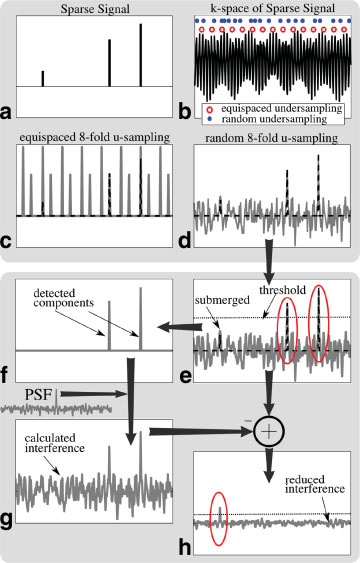
\includegraphics[width=\linewidth]{images/project with Wiem/fig-001.png}
    \caption{An intuitive reconstruction of a sparse signal from pseudo-random k-space undersampling. A sparse signal (a) is 8-fold undersampled in k -space (b). Equispaced undersampling results incoherent signal aliasing (c) that cannot be recovered. Pseudo-random undersampling results in incoherent aliasing (c). Strong signal components stick above the interference, are detected (e) and recovered (f) by thresholding. The interference of these components is computed (g) and subtracted (h), lowering the total interference level and enabling recovery of weaker components. Image and caption from~\cite{sparse}.}
    \label{fig:incoherence}
\end{figure}

\subsubsection{Measuring Coherence} 
In the following we introduce two tools to measure the coherence between samples: 
Point Spread Function (PSF) and Transform Point Spread Function (TPSF).
\begin{itemize}
    \item Point Spread Function (PSF):
    $$PSF(i,j)=e_{j}^{*}F_{u}^{*}F_{u}e_{i}$$
    measures contribution of a unit-intensity pixel at the $i^{th}$ position to a pixel at $j^{th}$ position  
    \item Transform Point Spread Function (TPSF):
    $$TPSF(i,j)=e_{j}^{*}\Psi F_{u}^{*}\Psi_{*} F_{u}e_{i}$$
    measures influence of a single transform
    coefficient to other transform coefficients. Here $F_{u}$ is the undersampled Fourier Operator, $\Psi$ is an orthogonal sparsifying matrix, $e_{i}$ and $e_{j}$ are basis vectors.
\end{itemize}
\begin{figure}
    \centering
    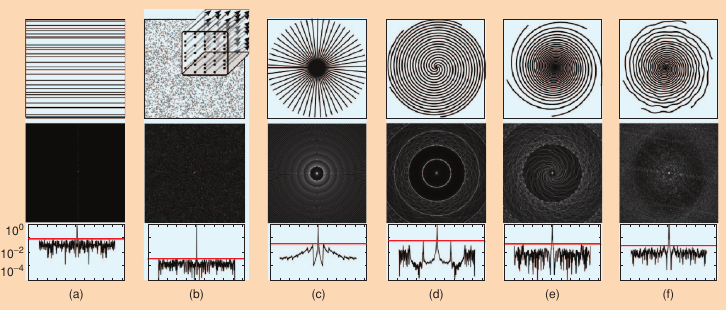
\includegraphics[width=\linewidth]{images/project with Wiem/non-cartesian-sampling.png}
    \caption{PSFs of various sampling trajectories: (a) random lines in 2-D, (b) random points in 2-D or cross-section of random lines in 3-D, (c) radial, (d) uniform spirals, (e) variable density spirals, and (f) variable density perturbed spirals. The height of the red lines measures coherence. Image and caption from~\cite{compressed}.}
    \label{fig:trajectories}
\end{figure}

\subsubsection{Variable Density Random Undersampling}
Our incoherence analysis assumes nonzero elements scattered randomly in the k-space in a sparse representation.  However, in natural images, most of the energy is concentrated around the origin of the k-space.
A uniform random distribution of samples in the spatial-frequency domain does not
take into account the energy distribution of MR images in k-space.   Therefore it makes more sense to opt for a nonuniform variable
density sampling matching energy distribution in k-space. Precisely, we should consider having more samples from the central part of the frequency domain and less highfrequency components. One possibility is sampling with density scaling according to a power of distance from the origin. Fig.~\ref{fig:trajectories} shows examples of physically feasible sampling patterns.

\fi

\section{Proximal Optimized Gradient Method}
Why is it faster than FISTA, and why is it optimal

D. Kim and J. A. Fessler, “Optimized first-order methods for smooth convex minimization,” Math. Program., vol. 159, no. 1, pp. 81–107, Sep. 2016, doi: 10.1007/s10107-015-0949-3.

\section{Decompositions}

\subsection{Low rank and Sparse}
C. Y. Lin and J. A. Fessler, “Efficient Dynamic Parallel MRI Reconstruction for the Low-Rank Plus Sparse Model,” IEEE Transactions on Computational Imaging, vol. 5, no. 1, pp. 17–26, Mar. 2019, doi: 10.1109/TCI.2018.2882089.

J. A. Fessler, “Optimization methods for MR image reconstruction (long version),” arXiv:1903.03510 [eess, math], Jun. 2019.

\subsection{Multiscale}

Ong's dissertation: “Low Dimensional Methods for High Dimensional Magnetic Resonance Imaging,” 2018.

F. Ong et al., “Extreme MRI: Large-Scale Volumetric Dynamic Imaging from Continuous Non-Gated Acquisitions,” arXiv:1909.13482 [physics], Dec. 2019.

Differences between Ong's dissertation and his "extreme MRI" preprint paper

\section{IRSL}
Iteratively reweighted Least Squares method

C. Kümmerle and C. M. Verdun, “Denoising and Completion of Structured Low-Rank Matrices via Iteratively Reweighted Least Squares,” arXiv:1811.07472 [cs, math], Nov. 2018.

Henry Adams, Lara Kassab, and Deanna Needell "An Iterative Method for Structured Matrix Completion"

\clearpage % You need \clearpage at the end of every chapter to force images included in this chapter to be rendered in somewhere else
\chapter{Implementation details}
% The Code of Studies and Exams recommends the following content for this chapter: "Presentation of used methodologies/technologies: In line with the topic of the dissertation, the professional background related to the solution and implementation of the task must be detailed."
% However, you are free to structure the content of your thesis as you want

\section{FunctionOperators package}
Describe this package what I created, and explain why was it useful.
\subsection{Objective}
\subsection{Features}

\section{Implementation of Sparse+Low Rank algorithms}
Re-implementation of Lin \& Fessler paper
\subsection{PINCAT dataset}
\subsection{Description of Algorithms in the article}

\section{Implementation of Multiscale Decomposition}

\subsection{NUFFT}
\paragraph{What is NUFFT}
\paragraph{Available solutions}
\paragraph{My implementation}

\subsection{Description of algorithm}

\subsection{Optimization possibilities}
\begin{enumerate}
    \item Batch-processing: compute NUFFT of all channels at once
    \item Parallelization:
    \begin{enumerate}
        \item NUFFT
        \item Algorithm
    \end{enumerate}
    \item GPU-specific optimizations:
    \begin{enumerate}
        \item Blocking operator might cause CPU bottleneck
    \end{enumerate}
\end{enumerate}

\subsection{Parallelization Solution}
Details how I made the code run parallel

\section{IRLS Implementation}

\subsection{Description of Algorithm}
\subsection{Implementation Details}

\clearpage % You need \clearpage at the end of every chapter to force images included in this chapter to be rendered in somewhere else

\chapter{Results}
% The Code of Studies and Exams recommends the following content for this chapter: "Evaluation, critical analysis of the implemented technical solutions, possibilities for further development."
% However, you are free to structure the content of your thesis as you want

\section{Sparse + Low Rank Algorithm}
\subsection{Running Speed and Memory Used}
\subsection{Readability}

\section{Multi-scale Algorithm}
\subsection{Running Speed and Memory Used}

\section{ILRS}
\subsection{Comparism with Sparse+Low Rank}
\paragraph{Running speed and memory requirement}
\paragraph{Convergence speed}
\paragraph{Robustness:} Effect of error on the input data
\paragraph{Recovery capability:} Can we reach the same accuracy on recovered image using less data?

\subsection{Comparism with Multi-scale}
\paragraph{Running speed and memory requirement}
\paragraph{Convergence speed}
\paragraph{Robustness:} Effect of error on the input data
\paragraph{Recovery capability:} Can we reach the same accuracy on recovered image using less data?

\clearpage % You need \clearpage at the end of every chapter to force images included in this chapter to be rendered in somewhere else
\chapter{Summary}
% The Code of Studies and Exams recommends the following content for this chapter:
% A summary of the problems solved compared to the objectives presented in the introduction and  in the Thesis Proposal Form. Opportunities to move forward, questions motivating the future works, outlook.
% However, you are free to structure the content of your thesis as you want

\section{Objectives}

In this thesis work, we considered the classic results as well as the recent advances within of the compressed sensing framework and their application to real life MR imaging. In particular, we closely examined two recent publications presenting state-of-the-art solutions combining conventional techniques with novel ideas. Afterwards, we implemented these algorithms along with a recently invented algorithm from the family of iteratively least squares methods that previously have not been applied to MRI setting yet. Finally, we compared these algorithm with respect to reconstruction power from massively undersampled data and noise tolerance.

\section{Achievements}
\section{Future Plans}

% Bibliography
\printbibliography
\addcontentsline{toc}{chapter}{Bibliography}

% Appendices -- if you don't have any, just delete the following two lines
%\appendix
%\chapter{Appendix}

Here you can present all the materials that helps the understanding of your work, but either 1) not your work, 2) not necessary to understanding, 3) simply just interesting things not directly related to your topic, or 4) your text already exceeded 120 pages, and need to make it shorter by moving parts to appendix... :D Anyway, if you have a large amount of images, code, or measurement data, it is required to insert them here rather than in chapters. You can have multiple appendices (possible separated into multiple files) according to the content to be attached.
